\documentclass[11pt,a4paper]{article}

\usepackage[margin=2.3cm]{geometry}
\usepackage{amsmath,amssymb,amsthm}
\usepackage{booktabs}
\usepackage{graphicx}
\usepackage{float}
\usepackage[numbers]{natbib}
\usepackage{hyperref}
\usepackage{xcolor}
\usepackage{enumitem}
\usepackage{array}
\usepackage{longtable}
\usepackage{caption}

\graphicspath{{figures/}{./}}
\hypersetup{colorlinks=true,linkcolor=blue,citecolor=blue,urlcolor=blue}
\captionsetup{font=small}

\newcounter{algobox}
\renewcommand{\thealgobox}{\arabic{algobox}}
\newcommand{\algcaption}[1]{\refstepcounter{algobox}\caption*{\textbf{Algorithm \thealgobox: }#1}}

\newtheorem{proposition}{Proposition}
\newtheorem{remark}{Remark}
\newtheorem{assumption}{Assumption}
\newtheorem{definition}{Definition}

\newcommand{\qos}{q}
\newcommand{\T}{\mathcal{T}}
\newcommand{\J}{\mathcal{J}}
\newcommand{\N}{\mathcal{N}}
\newcommand{\A}{\mathcal{A}}
\newcommand{\D}{D}
\newcommand{\U}{U}
\newcommand{\w}{\boldsymbol{w}}
\newcommand{\p}{\boldsymbol{p}}
\newcommand{\g}{\boldsymbol{g}}

\title{\textbf{A Three-Layer Nested Fixed-Point Candidate-Response Framework for Token Inference Services:\\
Wholesale Pricing, Capacity Allocation, and QoS Feedback\\under a Platform--Intermediary--User Structure}}

\author{Anonymous Author}
\date{}

\begin{document}

\maketitle

\begin{abstract}
\noindent
Large-model inference services exhibit significant time-of-day load fluctuations. Surge requests during peak periods push up time-to-first-token latency, timeout rates, and SLA violation risk, degrading billable service volume. This paper develops an auditable three-layer nested fixed-point candidate-response simulator for an inference-service market with one platform, multiple intermediaries, and users: the platform ranks time-differentiated wholesale-price candidates; intermediaries non-cooperatively choose retail prices and cross-period capacity allocations; users migrate among intermediary--period pairs based on price, period preference, native-period distribution, switching cost, and expected QoS; demand then feeds back to each layer through a QoS fixed point. On the theory side, we construct a finite congestion game at the user layer and prove the existence of a pure-strategy Nash equilibrium, then derive the logit stochastic user equilibrium linked to QoS via a damped fixed-point iteration. At the middle and upper layers, we place strict Stackelberg/SPE claims under additional regularity conditions as a theoretical boundary, and use a solver-consistent regret-bounded candidate response as the computable stability criterion connecting the model to the simulation.

On a synthetic benchmark, relative to dynamic pricing that ignores QoS degradation during the search phase, the three-layer QoS-aware strategy raises system profit from 8383.79 to 9525.12 (+13.61\%) and restores the minimum QoS from 0.8745 to 1.0000. Mechanism diagnostics further show that the full QoS cost and a quadratic congestion proxy above the degradation threshold produce almost identical candidate outcomes, indicating that the key mechanism under the current parameterization is not a particular QoS functional form but the internalization of congestion risk in intermediaries' retail-pricing and capacity-allocation decisions. At the same time, unconstrained revenue maximization drives user inclusive value down from 2.10 to $-0.52$; under a price-protection contract that caps both retail and wholesale prices at 0.80, platform revenue rises by 62.32\% relative to uniform retail while inclusive value rises modestly from 2.10 to 2.14. The main conclusion is therefore bounded: QoS/congestion-risk internalization can improve profit and the QoS floor under a specified candidate set and solver path, but simultaneous improvement in revenue, QoS, and user experience requires price protection, sufficient capacity, and calibration of real demand elasticities. The method's intended role is that of an offline mechanism simulator and policy-screening tool.
\end{abstract}

\noindent\textbf{Keywords:} Inference service; Token pricing; Intermediary; Nested fixed point; Candidate response; Solver-based regret; Cross-period capacity allocation; QoS feedback

% ============================================================
\section*{Nomenclature}
\label{sec:nomenclature}

\begin{longtable}{@{}p{0.28\textwidth}p{0.68\textwidth}@{}}
\toprule
Symbol & Meaning \\
\midrule
\endhead
\multicolumn{2}{l}{\textbf{Sets and Indices}} \\
$\T=\{1,\ldots,T\}$ & Set of time periods \\
$\J=\{1,\ldots,J\}$ & Set of intermediaries \\
$\N=\{1,\ldots,N\}$ & Set of users \\
$\A=\J\times\T$ & User choice set: intermediary--period pairs \\
$\A^+=(\J\cup\{0\})\times\T$ & Extended choice set with direct API channel \\
\midrule
\multicolumn{2}{l}{\textbf{Variables}} \\
$w_t$ & Wholesale price posted by the platform in period $t$ \\
$p_{j,t}$ & Retail price of intermediary $j$ in period $t$ \\
$g_{j,t}$ & Service capacity allocated by intermediary $j$ to period $t$ \\
$\D_{j,t}$ & Total demand flowing to intermediary $j$ in period $t$ \\
$q_{j,t}=\qos(\cdot)$ & QoS of intermediary $j$ in period $t$ (fraction effectively completed) \\
$p^D_t,g^D_t,\D^D_t,q^D_t$ & Retail price, capacity, demand, and QoS of the direct API channel in period $t$ \\
$u_{j,t}$ & Local utilization of intermediary $j$ in period $t$ \\
$s_{j,t}$ & Logit share of users choosing intermediary $j$ in period $t$ \\
$\Pi^P$ & Platform wholesale revenue \\
$\Pi^{P,+}$ & Platform payoff including direct API net earnings \\
$\Pi^I$ & Total intermediary profit \\
$\Pi^S$ & Total system profit \\
\midrule
\multicolumn{2}{l}{\textbf{Parameters}} \\
$h$ & Duration of one period (hours) \\
$G_j$ & Total capacity budget of intermediary $j$ \\
$\bar u$ & QoS degradation threshold utilization \\
$\kappa$ & QoS degradation steepness \\
$\alpha$ & User price sensitivity \\
$c_s$ & User cross-period switching cost \\
$c_g$ & Unit capacity cost \\
$c_q$ & Unit QoS degradation cost \\
$\bar F$ & Baseline flexible-demand scale \\
$a_t$ & User preference factor for period $t$ \\
$\pi_t$ & Native period distribution of users, $\sum_t\pi_t=1$ \\
$b_j$ & Brand/convenience factor of intermediary $j$ \\
$p_0$ & Baseline retail price \\
$\underline g$ & Positive floor for numerical capacity \\
\bottomrule
\caption{Model notation}
\label{tab:nomenclature}
\end{longtable}

% ============================================================
\section{Introduction}
\label{sec:intro}

\subsection{Background}

Large-model inference services have progressively shifted from offline batch processing to continuously running online services. Interactive chat, code generation, autonomous agents, offline evaluation, and periodic workflows exhibit distinct arrival patterns over the course of a day, creating substantial peak--valley differentials for GPU inference clusters. Systems research has shown that batching, resource sharing, memory management, and request scheduling jointly affect throughput, latency, and cost~\cite{crankshaw2017clipper,gujarati2020clockwork,romero2021infaas,yu2022orca,kwon2023pagedattention,agrawal2024sarathiserve}. When utilization approaches the capacity boundary, time-to-first-token latency, queuing time, and effective completion rates change rapidly; degradation of service quality directly reduces billable service volume and user satisfaction.

In the inference service market, the upstream platform (e.g., a model vendor or API provider that owns GPU clusters) must coordinate resource allocation among downstream intermediaries (agency platforms, industry service providers, API aggregators) and end users. In practice, however, the platform does not face all end users directly with a single retail price. Intermediaries, as independent profit-seeking entities, autonomously choose cross-period retail pricing and capacity allocation strategies based on the wholesale price. For example, API aggregators such as OpenRouter manage token budgets and model routing, which determines the service portfolio they offer to end users. The capacity allocation and retail pricing decisions of intermediaries, in turn, affect user migration across periods and intermediaries, altering local congestion states and QoS outcomes. Hence, faced with a complex system optimization problem involving multiple stakeholders, the platform needs to set internal time-differentiated wholesale prices for intermediaries. In real-world deployment, wholesale pricing typically cannot pursue short-run platform revenue alone; downstream profits, user experience, and SLA constraints must also be monitored. This paper first studies price pass-through under the platform-revenue objective and separately reports system profit, QoS, and user-welfare diagnostics in the experiments.

Against this background, a key research question arises: when inference services exhibit time-varying load and QoS degradation, how should a platform set time-differentiated wholesale prices so that, under intermediaries' autonomous optimization and users' free migration, a stable downstream response emerges, system profit improves, and the QoS floor rises? This question cannot be captured by single-layer profit maximization alone, because user demand is neither exogenous nor constant, intermediaries do not passively forward prices, and QoS is not a fixed parameter but an endogenous variable jointly determined by demand and capacity.

\textbf{Mechanism intuition.} For readers without a game-theoretic background, the core mechanism in this paper can be summarized in three steps. First, the wholesale price alters the marginal revenue of intermediaries serving requests in different periods. Second, intermediaries simultaneously adjust retail prices and capacity: they can screen out low-value requests by raising prices and shift capacity toward high-value periods close to their SLA boundary. Third, user migration changes local utilization, which in turn affects the effective settlement volume through the QoS function. This chain explains why QoS-aware strategies can raise both profit and QoS and why unconstrained revenue maximization harms user inclusive value: intermediaries have an incentive to raise retail prices to increase margins and simultaneously reduce congestion pressure.

\subsection{Related Work and Research Gap}
\label{sec:related_work}

Pricing for inference services in the existing literature is usually studied in conjunction with system scheduling or resource-management strategies~\cite{crankshaw2017clipper,yu2022orca,kwon2023pagedattention}. These works typically focus on two aspects: how to improve execution efficiency through batching, caching, and scheduling for a given set of requests, and cost--performance comparisons across different models or GPU clouds. Clipper, Clockwork, and INFaaS demonstrate the importance of model selection, scheduling, and resource management in ML serving~\cite{crankshaw2017clipper,gujarati2020clockwork,romero2021infaas}. Orca, PagedAttention, Sarathi-Serve, Splitwise, DistServe, and Vidur further propose system optimizations for batching, KV-cache management, prefill--decode interference, and simulator-based planning for large-model inference~\cite{yu2022orca,kwon2023pagedattention,agrawal2024sarathiserve,patel2024splitwise,zhong2024distserve,agrawal2024vidur}. These studies, however, answer the question of how to execute a given request set faster and generally do not embed demand migration, retail channels, and platform revenue in a single game-theoretic model.

In the pricing and market-mechanism direction, recent work has started to treat LLM inference service as a market system with both technical costs and economic responses, discussing inference cost, menu pricing, Stackelberg pricing/routing, and locational pricing~\cite{demirer2025emerging,erdil2025inference,bergemann2025menu,guo2026prillm,yan2026stackelberg,liu2026locational}. Yan et al.~\cite{yan2026stackelberg} propose a Stackelberg game that incorporates batching preferences and delay costs into a joint pricing--scaling optimization between an LLM inference service provider and its clients. Liu~\cite{liu2026locational} studies locational pricing and multi-market clearing for geographically distributed inference clusters. Work on menu pricing and token capacity contracts further shows that the user choice set and contractual structure affect service pricing outcomes~\cite{bergemann2025menu,xing2026tokenfutures}. These contributions demonstrate that LLM inference pricing is no longer merely a system-throughput optimization problem but one that requires simultaneously considering cost, demand response, service quality, and strategic interaction.

This paper narrows the research gap to a specific combinatorial problem: retaining within a single computable model the strategic intermediary, cross-period capacity allocation, user migration, and endogenous QoS feedback. Existing work typically concentrates on a subset---system scheduling, direct platform-to-user pricing, batching preferences, geographic market clearing, or contract menus. In settings involving agency platforms, API aggregators, and enterprise resellers, intermediaries also autonomously decide retail prices, model routing, and capacity budgets. If intermediaries are simplified to passive markup channels, the price pass-through chain wholesale $\to$ retail $\to$ user migration $\to$ local congestion $\to$ QoS feedback $\to$ effective settlement volume cannot be characterized. This paper therefore treats intermediaries as game-theoretic agents with independent strategy sets and embeds user choice and QoS degradation in the same three-layer response system.

Before turning to the game-theoretic modeling literature, real-time electricity pricing and demand-response studies provide a useful applied precedent, but not a direct template~\cite{schweppe1988spot,borenstein2005long,albadi2008summary,faruqui2010household,siano2014demand}. This literature shows how upstream real-time prices can guide downstream load migration across periods, and how such migration affects congestion, reliability, and system dispatch. Inference services share this price--load--reliability logic because both settings use prices to coordinate limited capacity and time-varying demand. The computable constraints, however, are different. Electricity markets are usually organized around generation constraints, network power flows, and market clearing, whereas inference-service quality is governed by local GPU utilization, latency, completion rate, and SLA compliance. Moreover, the intermediaries in this paper are not passive electricity consumers; they are channels that autonomously set retail prices and capacity budgets. Electricity pricing therefore serves here only as an applied precedent for the ``price signal--load migration--reliability feedback'' mechanism, while the model's computable objects are wholesale prices, retail prices, capacity budgets, logit user choice, and a QoS fixed point.

On the modeling side, the congestion-pricing and revenue-management literature provides the theoretical basis for coordinating price, limited capacity, and heterogeneous demand~\cite{vickrey1969congestion,gallego1994dynamic,elmaghraby2003dynamic,bitran2003overview,talluri2004revenue,phillips2005pricing}. Building on that basis, this paper combines congestion games, random-utility discrete-choice models, and logit equilibrium, with the limit passage from finite-player games to continuous demand response as the theoretical backbone~\cite{rosenthal1973class,monderer1996potential,wardrop1952some,sandholm2010population,mcfadden1974conditional,train2009discrete}. Connecting the existence proof of a PSNE in a potential game with the differentiable logit SUE and defining a checkable candidate response within a three-layer nested fixed-point system provides an explicitly bounded yet computable simulation framework for cross-period pricing of inference services.

\subsection{Contributions and Organization}

To address the above research gap, this paper studies a three-layer token-inference service market with a single platform, multiple intermediaries, and heterogeneous users, incorporating the QoS-degradation feedback chain while accounting for multi-stakeholder game-theoretic relationships and intermediaries' strategic degrees of freedom. The main contributions are as follows.

\begin{enumerate}[leftmargin=2em]
\item \textbf{Offline nested fixed-point mechanism simulator with QoS/congestion-risk internalization.}
  Unlike prior work that treats intermediaries as passive forwarding channels or QoS as a fixed parameter, our model establishes the feedback chain wholesale prices $\to$ intermediary retail prices and capacity allocation $\to$ user migration $\to$ local congestion $\to$ QoS feedback $\to$ profit. The framework is not positioned as a proof that three-layer markets are generally optimal. Instead, it provides an auditable offline simulator for screening wholesale--retail--capacity mechanisms under a specified wholesale-price candidate set, solver path, and QoS function.

\item \textbf{Solution-concept hierarchy, user-layer guarantees, and solver-consistent candidate response.}
At the user layer we construct a finite congestion game with a Rosenthal potential function, prove the existence of a pure-strategy Nash equilibrium (PSNE), derive the logit stochastic user equilibrium (SUE) from the random-utility model, and explain the theoretical link from finite-player equilibria to the large-population logit response. At the intermediary layer we write the profit function containing retail revenue, wholesale cost, capacity cost, and QoS-degradation cost, and derive first-order conditions and KKT conditions for capacity allocation. Because logit demand and QoS feedback can make the middle-layer profit numerically non-convex with flat local structure, we explicitly separate the roles of PSNE, the SUE--QoS fixed point, solver-based regret, and platform candidate ranking. Strict SPE existence is placed under additional regularity conditions (quasiconcavity and upper semi-continuity), and the numerical response is reported as a solver-consistent candidate rather than a global Nash or global SPE certificate.

  \item \textbf{Reproducible mechanism findings and user-experience boundaries.}
  On a synthetic benchmark we implement five strategy comparisons (uniform retail, platform direct, single intermediary, dynamic pricing without QoS awareness, three-layer QoS-aware pricing) and systematically report platform wholesale revenue, intermediary profit, system profit, minimum QoS, peak utilization, solver-based regret, and user inclusive value. The core experimental finding is not a mere book-profit improvement: the QoS cost and a congestion proxy both work mainly by making intermediaries internalize congestion risk and recover effective settlement volume; unconstrained three-layer revenue maximization improves QoS yet depresses user utility. Price-protection contracts and the direct API outside option can mitigate this problem within bounded parameter regions. To avoid extrapolating a single synthetic scenario to a production conclusion, supplemental experiments are grouped into mechanism attribution and finite-user bridging, algorithmic and parameter robustness, vLLM-measured QoS and measurement-driven arrival replay, and user protection and direct-API sensitivity---delimiting the parameter regions in which revenue, QoS, and user-experience improvements can hold simultaneously.
\end{enumerate}

The remainder of the paper is organized following the three-layer modeling order. Section~\ref{sec:problem} presents the problem description and multi-stakeholder information interactions. Section~\ref{sec:formulation} gives the mathematical models of the upper platform, middle intermediaries, and lower users, together with the three-layer candidate-response definition. Section~\ref{sec:solution} describes the iterative computation of the candidate response. Section~\ref{sec:case_study} reports the case-study results and discussion. Section~\ref{sec:conclusion} concludes the paper.

% ============================================================
\section{Problem Description}
\label{sec:problem}

In an inference-service market, multiple autonomous agents participate in token transactions with interdependent yet conflicting economic objectives. We refer to these agents as stakeholders. Concretely, as illustrated in Figure~\ref{fig:three_layer_framework}, we consider a single platform that owns or leases upstream GPU inference capacity and aggregates three categories of downstream stakeholders: multiple intermediaries (agency platforms, industry-application service providers, API aggregators, or resellers) and end users. Intermediaries sit between the platform and users: they purchase inference capacity from the platform, repackage it, and sell it to end users. Users have heterogeneous period preferences, switching costs, and price sensitivities and can migrate among multiple intermediaries and periods. The platform and intermediaries transact tokens at wholesale prices; intermediaries and users transact at retail prices. The platform, intermediaries, and users are assumed to belong to distinct stakeholder groups, each making independent decisions.

This multi-stakeholder setting naturally generates conflicts of interest. The platform prefers to raise wholesale prices to increase upstream revenue, but excessively high wholesale prices squeeze intermediary profit margins, leading to higher retail prices and demand loss. Intermediaries wish to raise retail prices and capacity utilization to earn higher margins, but excessive short-run profit seeking creates local congestion, lowers QoS, and reduces effective settlement volume, in turn harming their own profit. Users wish to select the intermediary--period pair with low price, good preference match, and high QoS, but the concentration of individual choices on the same period alters the congestion state and feeds back to affect all users choosing that pair. The platform's wholesale price influences intermediary profit margins; intermediary retail prices and capacity affect user migration; user migration alters local congestion; QoS changes effective service volume and profit, which in turn feeds back to the upper-layer pricing. These interconnected decisions form a complex layered interaction that cannot be described by a single-layer optimization model.

Hence the key research challenge is to determine: how should the platform design time-differentiated wholesale prices and intermediary scheduling strategies such that, when all stakeholders pursue their individual objectives, the final outcome constitutes a stable candidate response with no significant unilateral improvement within the scope of a given solver's search? Such a response can provide a checkable price--capacity relation for inference-service interactions among stakeholders, while its welfare implications still depend on the platform's objective function and additional participation constraints.

To address this challenge, this paper proposes a three-layer nested fixed-point candidate-response framework that explicitly models the layered decision structure among stakeholders. As shown in Figure~\ref{fig:three_layer_framework}, the upper layer instantiates the platform as model vendors such as DeepSeek, Claude, and GPT/OpenAI together with an upstream API supply network; the middle layer draws intermediaries as OpenRouter-style API aggregators, enterprise resellers, and application platforms. The platform posts time-differentiated wholesale prices $\w$; intermediaries observe the wholesale prices and simultaneously choose retail prices $\p$ and cross-period capacity allocations $\g$; users observe the retail prices and expected QoS and choose intermediary--period pairs $(j,t)$. Under non-convex middle-layer responses, user--QoS fixed points, and a finite wholesale-price candidate set, this paper employs the three-layer structure as an offline mechanism-simulation and policy-screening framework rather than interpreting the numerical output as a global SPE in a continuous strategy space.

\begin{figure}[H]
\centering
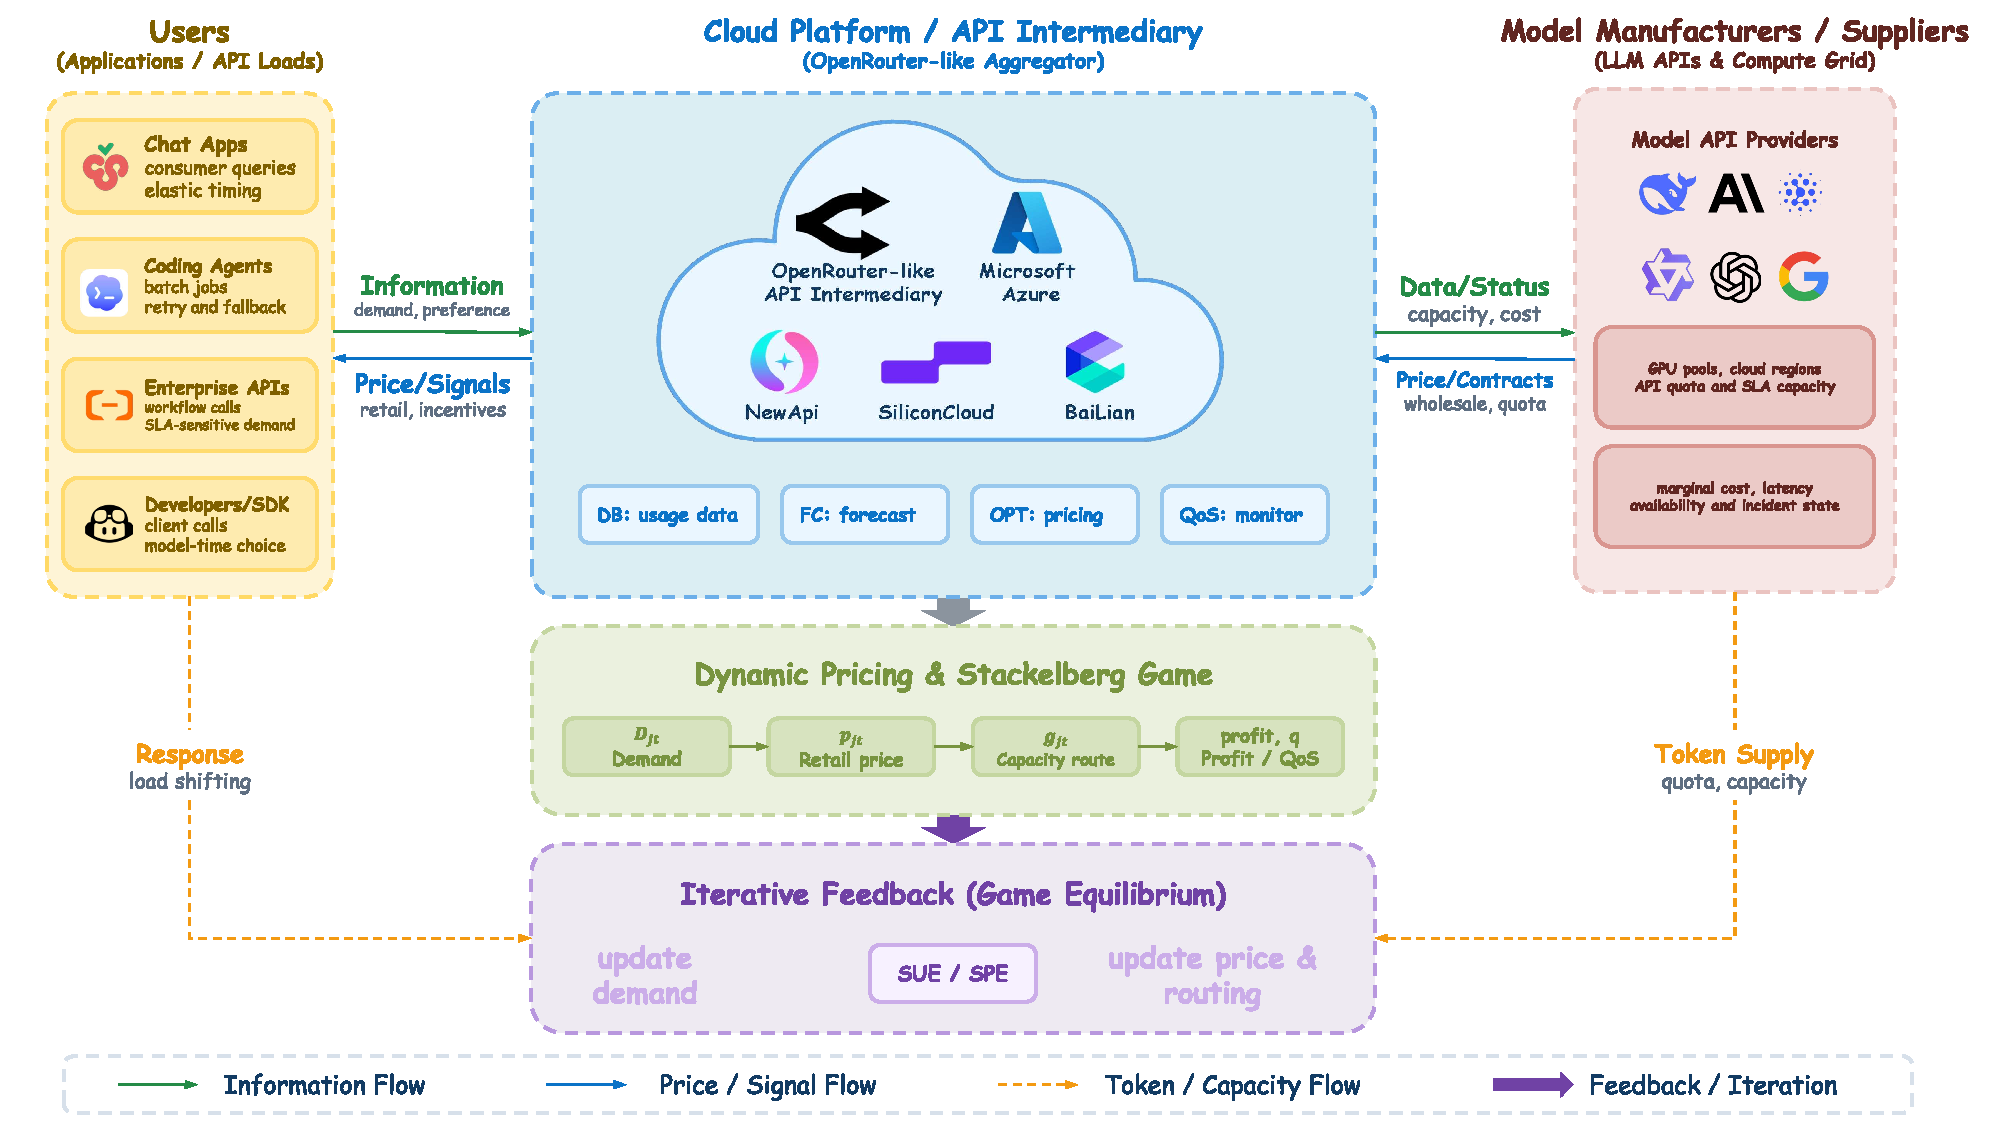
\includegraphics[width=\textwidth]{figures/three_layer_game_framework.pdf}
\caption{Interconnected three-layer game among model vendors, API intermediaries, and applications/users. Upstream model vendors include API suppliers such as DeepSeek, Claude, and GPT/OpenAI; OpenRouter-style aggregators and enterprise resellers choose model routing, capacity, and retail prices; users migrate among intermediary--period pairs $(j,t)$, and intermediaries route demand to upstream model APIs. Demand creates local utilization, and QoS in turn feeds back to billable service volume, profit, and price updates.}
\label{fig:three_layer_framework}
\end{figure}

% ============================================================
\section{Mathematical Model}
\label{sec:formulation}

Let a day be divided into $T$ periods $\T=\{1,\ldots,T\}$, let the set of intermediaries be $\J=\{1,\ldots,J\}$, and let the set of users be $\N=\{1,\ldots,N\}$. The platform posts a wholesale-price vector $\w=(w_1,\ldots,w_T)$. Intermediary $j$ allocates serviceable capacity $g_{j,t}\ge \underline g>0$ to period $t$ and posts a retail price $p_{j,t}$. Each user chooses an intermediary--period pair $(j,t)$. Service quality is determined by the local load of the intermediary:
\begin{equation}
  u_{j,t}=\frac{\D_{j,t}}{g_{j,t}},\qquad
  q_{j,t}=\qos(u_{j,t})=
  \begin{cases}
    1, & u_{j,t}\le \bar u,\\[2pt]
    \exp[-\kappa(u_{j,t}-\bar u)^2], & u_{j,t}>\bar u.
  \end{cases}
  \label{eq:qos}
\end{equation}
where $\D_{j,t}$ is the total demand flowing to intermediary $j$ in period $t$. If $g_{j,t}$ is too small or $\D_{j,t}$ too large, $q_{j,t}$ decreases, indicating that the fraction of service effectively completed declines.

Platform revenue, intermediary profit, and system profit are respectively
\begin{align}
  \Pi^P(\w,\p,\g)
  &=h\sum_{j\in\J}\sum_{t\in\T} w_t\D_{j,t}q_{j,t}, \label{eq:platform_profit}\\
  \Pi^I(\w,\p,\g)
  &=h\sum_{j,t}(p_{j,t}-w_t)\D_{j,t}q_{j,t}
    -h\sum_{j,t}c_g g_{j,t}
    -h\sum_{j,t}c_q(1-q_{j,t})\D_{j,t}, \label{eq:intermediary_profit}\\
  \Pi^S(\w,\p,\g)&=\Pi^P+\Pi^I. \label{eq:system_profit}
\end{align}
This definition reports the platform's wholesale revenue and the intermediaries' retail margins separately. QoS degradation reduces both the effective settlement volume and, through $c_q$, accounts for SLA violations, user churn, or service-compensation costs. This paper interprets the two terms as distinct contractual channels: the former corresponds to settlement by effectively completed volume, and the latter to service compensation or future churn cost. If a real contract uses only one of these accounting rules, $c_q$ should be re-estimated and the billing rule should be ablated before using the numerical values as profit predictions.

In an extension where users can simultaneously choose the vendor's direct API, the user action set becomes
\begin{equation}
  \A^+=(\J\cup\{0\})\times\T,
  \label{eq:direct_api_action_set}
\end{equation}
where $j=0$ denotes the platform's self-operated direct API channel. This channel has a direct retail price $p^D_t$ and direct capacity $g^D_t$, entering the user logit choice together with the intermediary channels. The platform payoff can then be written as
\begin{equation}
  \Pi^{P,+}
  =h\sum_{j\in\J}\sum_{t\in\T}w_t\D_{j,t}q_{j,t}
  +h\sum_{t\in\T}\left[
    p^D_t\D^D_tq^D_t-c_g g^D_t-c_q(1-q^D_t)\D^D_t
  \right],
  \label{eq:direct_platform_payoff}
\end{equation}
where the first term is the platform's wholesale revenue from intermediaries and the second term is the net earnings of the direct API channel. Intermediary profit is still computed only over $j\in\J$. We treat this extension as a supplementary experiment to test whether the direct API as a user outside option constrains intermediary pricing and how it affects user experience. In this extension the normalization scope of Eq.~\eqref{eq:logit_share} and the share summation in Eq.~\eqref{eq:demand} are extended to $\J\cup\{0\}$. Numerical experiments first fix $p^D_t$ and $g^D_t$ to examine the constraining role of the direct channel as an outside option, and then conduct price--capacity sweeps to test the parameter boundary of this constraining effect; this paper does not interpret the extension as a joint optimal design of direct price and capacity.

\subsection{Upper Layer: Platform Wholesale Pricing}
\label{sec:upper_platform}

The platform at the upper layer chooses $\w\in[\underline w,\overline w]^T$. It does not directly control downstream demand but anticipates the effective service volume $\D_{j,t}q_{j,t}$ formed after intermediary and user responses. The platform's problem is
\begin{equation}
  \max_{\w\in[\underline w,\overline w]^T}\;
  \Pi^P(\w,\p^*(\w),\g^*(\w)),
  \label{eq:platform_problem}
\end{equation}
where $(\p^*(\w),\g^*(\w))$ denotes an intermediary-layer response that can be selected under additional regularity conditions, and user demand is given by the lower-layer choice model. Equation~\eqref{eq:platform_problem} clarifies that the platform adjusts wholesale prices, not terminal retail prices or user choice itself. In the numerical instances of this paper, however, the intermediary response is jointly determined by non-convex optimization and a user--QoS fixed point; the actually solved object is therefore the candidate-response set and platform candidate ranking defined in Section~\ref{sec:fixed_point}, not an analytic single-valued response function.

Equation~\eqref{eq:platform_problem} describes a platform-revenue objective, not a social-welfare objective. If an operator wishes to explicitly incorporate user welfare or downstream participation constraints into the upper-layer decision, constraints such as
\begin{equation}
  \Pi^I_j(\w,x)\ge \Pi^{I,\mathrm{ref}}_j,\quad
  W^U(\p,\g)\ge W^{U,\mathrm{ref}},\quad
  \bar q_{\mathrm{active}}\ge q_{\mathrm{SLA}},
  \label{eq:deployment_constraints}
\end{equation}
can be added to the platform layer, where $W^U(\p,\g)=\log\sum_{j,t}\exp(z_{j,t})$ is the user-side inclusive value of the logit model and $\bar q_{\mathrm{active}}$ denotes a quality-of-service metric over active demand units. The main experiments in this paper first use platform revenue as the candidate-ranking objective, then separately report system profit, intermediary profit, QoS, and platform candidate-reference searches in the experimental section, so as to identify whether the platform objective and the system objective exhibit tension.

\subsection{Middle Layer: Intermediary Retail Pricing and Capacity Allocation}
\label{sec:middle_intermediary}

Given the platform's wholesale price $\w$, intermediary $j$ observes the upper-layer price and chooses $\g_j=(g_{j,1},\ldots,g_{j,T})$ and $\p_j=(p_{j,1},\ldots,p_{j,T})$, satisfying
\begin{equation}
  \sum_{t=1}^{T}g_{j,t}=G_j,\qquad g_{j,t}\ge \underline g,\qquad
  p_{j,t}\in[\underline p,\overline p].
  \label{eq:capacity_constraint}
\end{equation}
where $\underline g$ is a positive capacity floor to avoid $D/g$ singularities, requiring $G_j\ge T\underline g$. In the numerical implementation we take $\underline g=10^{-6}$, which is negligible relative to the magnitude of $G_j$.

With other intermediaries' strategies fixed, the best response of intermediary $j$ is
\begin{equation}
  \mathcal{BR}_j(\w,x_{-j})=
  \arg\max_{x_j\in\Omega_j}\;
  \left[
  h\sum_{t}(p_{j,t}-w_t)\D_{j,t}q_{j,t}
  -h\sum_t c_g g_{j,t}
  -h\sum_t c_q(1-q_{j,t})\D_{j,t}
  \right],
  \label{eq:broker_problem}
\end{equation}
where $x_j=(\p_j,\g_j)$, $x_{-j}$ denotes the strategies of intermediaries other than $j$, and $\Omega_j$ is given by Eq.~\eqref{eq:capacity_constraint}. Given $\w$, if no intermediary can achieve a unilateral profit improvement exceeding $\epsilon_N$ under the best-response solver specified in this paper, then the strategy profile satisfies the middle-layer candidate-response condition of Definition~\ref{def:solver_regret_candidate}.

This objective function contains retail revenue, wholesale cost, capacity cost, and QoS loss cost. Unlike a price-only model, the intermediary must also decide how to allocate capacity across periods. Too little capacity raises utilization and degrades QoS; too much capacity increases idle cost.

\subsubsection{Retail-price first-order conditions}

Let $M_{j,t}=(p_{j,t}-w_t)q_{j,t}-c_q(1-q_{j,t})$ denote the effective margin per unit of demand. Ignoring boundary conditions, the first-order condition for the retail price is
\begin{equation}
  \frac{\partial\Pi^I_j}{\partial p_{j,t}}
  =h\left[
  \D_{j,t}q_{j,t}
  +M_{j,t}\frac{\partial \D_{j,t}}{\partial p_{j,t}}
  +(p_{j,t}-w_t+c_q)\D_{j,t}\frac{\partial q_{j,t}}{\partial p_{j,t}}
  \right]=0.
  \label{eq:retail_foc}
\end{equation}
The first term is the direct revenue from raising the retail price, the second is the loss from reduced demand due to the price increase, and the third is the indirect effect of demand changes on QoS through utilization.

\subsubsection{Capacity-allocation KKT conditions}

The Lagrangian for capacity allocation is
\begin{equation}
  \mathcal{L}_j=\Pi^I_j+\lambda_j\left(G_j-\sum_t g_{j,t}\right)
  +\sum_t \mu_{j,t}(g_{j,t}-\underline g).
  \label{eq:broker_lagrangian}
\end{equation}
The KKT conditions are
\begin{align}
  \frac{\partial\Pi^I_j}{\partial g_{j,t}}-\lambda_j+\mu_{j,t}&=0,
  \label{eq:kkt_stationarity}\\
  \sum_t g_{j,t}=G_j,\quad g_{j,t}\ge \underline g,\quad \mu_{j,t}\ge 0,\quad
  \mu_{j,t}(g_{j,t}-\underline g)&=0. \label{eq:kkt_complementarity}
\end{align}
Because $q_{j,t}=\qos(\D_{j,t}/g_{j,t})$, increasing capacity lowers utilization and raises QoS. When $g_{j,t}>\underline g$, $\mu_{j,t}=0$, and Eq.~\eqref{eq:kkt_stationarity} indicates that the marginal benefit of capacity in each active period equals the common shadow price $\lambda_j$. This yields the economic interpretation of joint capacity and price scheduling: capacity is more valuable in peak periods, but excessively high retail prices drive users to other intermediaries or other periods.

\subsection{Lower Layer: User Choice, Congestion Game, and Logit Equilibrium}
\label{sec:lower_user}

\subsubsection{Finite-player congestion game}

The user-layer choice set is $\A=\J\times\T$. User $i$'s action is $a_i=(j_i,t_i)\in\A$. Given the actions $a_{-i}$ of other users, let $n_{j,t}(a)$ denote the number of users choosing $(j,t)$. User $i$'s deterministic payoff when choosing $(j,t)$ is
\begin{equation}
  r_i(j,t;n_{j,t}) =
  \log(b_j+\varepsilon)+\log(a_t+\varepsilon)
  -\alpha\left[p_{j,t}+c_s\mathbf{1}[t\ne \tau_i]-p_0\right]
  -\delta\left[1-\qos\!\left(\frac{n_{j,t}}{\bar g_{j,t}}\right)\right],
  \label{eq:finite_payoff}
\end{equation}
where $b_j$ is the brand or convenience of intermediary $j$, $a_t$ is the period preference, $\tau_i$ is user $i$'s native preferred period, $c_s$ is the switching cost, and $\bar g_{j,t}$ is the discrete capacity scale in the finite game. The last term captures congestion disutility: when more users choose the same intermediary and period, service quality drops.

\begin{proposition}[Existence of a PSNE at the user layer]
\label{prop:psne}
The finite-user game defined by Eq.~\eqref{eq:finite_payoff} is an exact potential game; hence a pure-strategy Nash equilibrium exists.
\end{proposition}

\begin{proof}
Construct the Rosenthal-type potential function
\begin{align}
  \Phi(a)=
  &\sum_{i\in\N}
  \left[\log(b_{j_i}+\varepsilon)+\log(a_{t_i}+\varepsilon)
  -\alpha\left(p_{j_i,t_i}+c_s\mathbf{1}[t_i\ne \tau_i]-p_0\right)\right] \nonumber\\
  &-\delta\sum_{j\in\J}\sum_{t\in\T}
  \sum_{k=1}^{n_{j,t}(a)}
  \left[1-\qos\!\left(\frac{k}{\bar g_{j,t}}\right)\right].
  \label{eq:potential}
\end{align}
Consider a unilateral deviation of user $i$ from $a_i=(j,t)$ to $a_i'=(j',t')$. All terms involving other users cancel exactly in $\Phi(a_i',a_{-i})-\Phi(a_i,a_{-i})$. The first line leaves only the change in user $i$'s own non-congestion payoff. In the second line, the original pair $(j,t)$ loses one term $1-\qos(n_{j,t}/\bar g_{j,t})$, and the new pair $(j',t')$ gains one term $1-\qos((n_{j',t'}+1)/\bar g_{j',t'})$. Hence
\[
\Phi(a_i',a_{-i})-\Phi(a_i,a_{-i})
=r_i(a_i';n_{j',t'}+1)-r_i(a_i;n_{j,t}).
\]
The change in the potential function equals the change in the deviating user's payoff, so the game is an exact potential game. Every finite exact potential game has at least one action profile that locally maximizes the potential function; that profile is a pure-strategy Nash equilibrium~\cite{rosenthal1973class,monderer1996potential}.
\end{proof}

\subsubsection{Random utility and logit SUE derivation}

The finite PSNE provides a micro-foundation of individual rationality, but directly enumerating $|\A|^N$ action profiles is computationally infeasible. Under a large-population approximation we use a random-utility model to obtain the differentiable aggregate response. The utility of user $i$ for pair $(j,t)$ is
\begin{equation}
  U_{i,j,t}=z_{j,t}+\epsilon_{i,j,t},
  \quad
  z_{j,t}=\log(b_j+\varepsilon)+\log(a_t+\varepsilon)
  -\alpha\left[p_{j,t}+c_s(1-\pi_t)-p_0\right]
  -\gamma[1-q_{j,t}],
  \label{eq:random_utility}
\end{equation}
where $\epsilon_{i,j,t}$ is i.i.d.\ Gumbel noise and $\pi_t=\Pr(\tau_i=t)$ is the distribution of users' native preferred periods. The switching term in Eq.~\eqref{eq:random_utility} replaces the individual native preference $\tau_i$ not with the average period affinity $a_t$ but with the population expectation of the finite-user switching cost $c_s\mathbf{1}[t\ne\tau_i]$:
\begin{equation}
  \mathbb{E}_{\tau_i\sim\pi}\!\left[c_s\mathbf{1}[t\ne\tau_i]\right]
  =c_s\sum_{\tau\in\T}\pi_\tau\mathbf{1}[t\ne\tau]
  =c_s(1-\pi_t).
  \label{eq:aggregate_switch_cost}
\end{equation}
In the numerical experiments, $\pi_t$ is set to the normalized period affinities as the native-period distribution; if real retention, booking, or enterprise-call logs are available, $\pi_t$ should be estimated directly from users' native call periods, or further refined with grouped distributions $\pi_{m,t}$ to capture differences among enterprise users, individual developers, and agency users. This aggregate formulation compresses the heterogeneity of native periods into a single population expectation and may therefore understate the concentration of native peak-period users and the associated local-congestion risk. A finer individual or grouped logit model could be written as $z_{m,j,t}$, where users of class $m$ use their own switching-cost vector $c_s\mathbf{1}[t\ne\tau_m]$; this paper adopts Eq.~\eqref{eq:aggregate_switch_cost} to keep the three-layer response computable and lists this simplification as a limitation that requires real-log calibration.

By the extreme-value property of the Gumbel distribution, the probability that a user chooses $(j,t)$ is
\begin{equation}
  s_{j,t}=\Pr\{(j,t)=\arg\max_{(k,\tau)\in\A}U_{i,k,\tau}\}
  =\frac{\exp(z_{j,t})}{\sum_{k\in\J}\sum_{\tau\in\T}\exp(z_{k,\tau})}.
  \label{eq:logit_share}
\end{equation}
Equation~\eqref{eq:logit_share} is the user-layer logit stochastic user equilibrium (SUE). Given retail prices, capacity, and QoS, the share matrix $\boldsymbol{s}$ is unique; if the QoS feedback enters the utility, then $s_{j,t}$, $\D_{j,t}$, and $q_{j,t}$ jointly constitute a fixed point:
\begin{align}
  \D_{j,t}&=\bar F\,m(\p)\,s_{j,t}
  +\bar R_t\,\sigma[\beta(v_r-p_{j,t})]\sum_{k\in\J}s_{k,t}, \label{eq:demand}\\
  q_{j,t}&=\qos(\D_{j,t}/g_{j,t}). \label{eq:qos_fixed}
\end{align}
In Eq.~\eqref{eq:demand}, the first term represents elastic demand that can be affected by price and channel choice, with $m(\p)$ a market-size factor that expands as the average retail price falls; the second term represents period-specific rigid or replay demand, where $\bar R_t$ is the base arrival intensity for that period and $\sigma[\beta(v_r-p_{j,t})]$ is the fraction lost when the price exceeds the reservation value $v_r$, with $\sum_k s_{k,t}$ distributing that period's demand across intermediaries according to user choice shares. This two-part structure serves simulation: it simultaneously retains migratable elastic demand and rigid arrivals with a period shape. Its economic parameters remain synthetic; for production pricing they should be recalibrated with real request traces, willingness-to-pay, and churn behavior.

Under the standard population-game approximation the empirical distribution of the finite potential game can be approximated by continuous demand shares; upon further adding Gumbel random preferences the aggregate choice probabilities are given by Eq.~\eqref{eq:logit_share}. This paper uses this modeling chain to connect the existence of a finite-user PSNE with the computable logit aggregate demand function, without interpreting the numerical experiments as an explicit enumeration of per-user PSNE profiles.

\begin{proposition}[Existence of the user-layer SUE fixed point]
\label{prop:sue_fixed_point}
Given any feasible retail price $\p$ and positive capacity $\g$, if the demand function $\D(\boldsymbol{s},\p)$ is continuous and the QoS function $\qos(u)$ is continuous with values in $[0,1]$, then the coupled system of Eqs.~\eqref{eq:logit_share}--\eqref{eq:qos_fixed} has at least one user-layer SUE--QoS fixed point. If, furthermore, there exists a constant $L_\qos L_D L_s<1$, where $L_s$ is the Lipschitz constant of the logit share with respect to the QoS vector, $L_D$ the Lipschitz constant of demand with respect to shares, and $L_\qos$ the Lipschitz constant of QoS with respect to demand, then the fixed point is unique and the damped iteration converges at a linear rate.
\end{proposition}

\begin{proof}
Let $\mathcal{Q}=[0,1]^{J\times T}$. For any $q\in\mathcal{Q}$, Eq.~\eqref{eq:logit_share} yields a continuous share $\boldsymbol{s}(q)$, Eq.~\eqref{eq:demand} yields a continuous demand $\D(\boldsymbol{s}(q),\p)$, and Eq.~\eqref{eq:qos_fixed} yields a new QoS vector $\widehat q(q)=\qos(\D/g)$. Because $\qos(\cdot)\in[0,1]$, the mapping $\widehat q:\mathcal{Q}\to\mathcal{Q}$ is a continuous self-map, and $\mathcal{Q}$ is nonempty, compact, and convex. By Brouwer's fixed-point theorem, there exists at least one $q^*$ such that $q^*=\widehat q(q^*)$. If the composition's Lipschitz constant is less than~1, then $\widehat q$ is a contraction mapping, and Banach's fixed-point theorem gives uniqueness and iterative convergence. The damped update $q^{\ell+1}=\eta\widehat q(q^\ell)+(1-\eta)q^\ell$ remains a contraction under the same condition and therefore converges to the same fixed point.
\end{proof}

\subsection{Three-Layer Nested Fixed-Point Candidate-Response Definition}
\label{sec:three_level_game}

We assume that all stakeholders considered in this paper---the platform, intermediaries, and users---are self-interested agents, each optimizing its own profit or utility objective. This multi-stakeholder layered setting can be organized as a sequential response computation, but because user choice, demand, and QoS form an internal fixed point, the middle-layer response is generally not an analytic single-valued function. The three-layer decision process can therefore be written as the following nested candidate-response framework. The platform first posts wholesale prices $\w\in[\underline w,\overline w]^T$; each intermediary $j$, upon observing $\w$, chooses $(\p_j,\g_j)$ satisfying Eq.~\eqref{eq:capacity_constraint}; users finally choose $(j,t)\in\A$, forming the demand matrix $\D(\w,\p,\g)$ and the QoS matrix $q(\D,\g)$. When the user layer reaches an SUE--QoS fixed point, the intermediary layer reaches a solver-consistent regret-bounded candidate response, and the platform completes the revenue ranking within a preset wholesale-price candidate set, we refer to the overall configuration as a three-layer candidate strategy response.

To avoid mixing solution concepts, this paper uses equilibrium language only at the layer where it is justified. The finite-user PSNE provides the microfoundation for the congestion game; the logit SUE--QoS fixed point is the user-layer response actually invoked by the continuous-demand simulator; the intermediary layer reports only solver-consistent unilateral-improvement diagnostics; and the platform layer ranks a finite wholesale-price candidate set. Table~\ref{tab:solution_concept_hierarchy} summarizes what each concept supports and what it does not support. The overall numerical object is a three-layer nested fixed-point candidate response, not an unqualified global Stackelberg equilibrium.

\begin{table}[H]
\centering
\caption{Solution-concept hierarchy and interpretation boundaries}
\label{tab:solution_concept_hierarchy}
\small
\begin{tabular}{@{}>{\raggedright\arraybackslash}p{0.15\textwidth}>{\raggedright\arraybackslash}p{0.20\textwidth}>{\raggedright\arraybackslash}p{0.27\textwidth}>{\raggedright\arraybackslash}p{0.25\textwidth}@{}}
\toprule
Layer & Concept used & Role in this paper & Claim not supported \\
\midrule
Finite user layer & PSNE & Provides a stable microfoundation for the individual congestion game & Not the final response used in the continuous-demand simulator \\
Continuous user layer & Logit SUE--QoS fixed point & Gives the user demand and QoS response embedded in every payoff evaluation & Does not guarantee uniqueness or global convergence under all parameters \\
Intermediary layer & Solver-based regret-bounded candidate response & Checks whether algorithm $\mathcal{A}$ can still find a significant unilateral improvement & Not a standard $\epsilon$-Nash certificate in the non-convex continuous strategy space \\
Platform layer & Finite candidate-set revenue ranking & Selects the returned response with the highest platform revenue within $\mathcal{W}_K$ & Not a global leader optimum over the continuous wholesale-price space \\
Overall object & Nested fixed-point candidate response & Connects the user fixed point, middle-layer candidate response, and platform candidate ranking & Strict SPE interpretation requires additional regularity conditions \\
\bottomrule
\end{tabular}
\end{table}

In the numerical instances of this paper, the intermediary profit function includes logit demand, QoS feedback, price-box constraints, and a capacity simplex constraint; the profit sections in Section~\ref{sec:reviewer_response_diagnostics} further show multiple shallow local peaks in the capacity direction. Hence this paper does not phrase the middle- and upper-layer numerical responses as strict global SPE, but instead adopts the following computational stability criterion.

\begin{definition}[Solver-consistent regret-bounded candidate response]
\label{def:solver_regret_candidate}
Given a platform wholesale price $\w$ and a middle-layer strategy profile $x=(x_1,\ldots,x_J)$ with $x_j=(\p_j,\g_j)$, let $\widehat{\mathcal{BR}}_j(\w,x_{-j};\mathcal{A})$ be intermediary $j$'s unilateral response returned by algorithm $\mathcal{A}$. In the numerical implementation, $\mathcal{A}$ is the bounded best-response routine after specifying initialization, bounds, SLSQP settings, the damped fixed-point solver, and stopping criteria, where every objective evaluation embeds the user-layer SUE--QoS fixed point. Define the reported solver regret as
\begin{equation}
  \widehat R_j(x;\w)=
  \max\left\{
  \Pi^I_j(\w,\widehat{\mathcal{BR}}_j(\w,x_{-j};\mathcal{A}),x_{-j})
  -\Pi^I_j(\w,x_j,x_{-j}),\,0
  \right\}.
  \label{eq:solver_reported_regret}
\end{equation}
If $\max_{j\in\J}\widehat R_j(x;\w)\le \epsilon_N$, then $x$ is called a solver-consistent regret-bounded candidate response under $\w$. We set $\epsilon_N=10^{-3}$.
\end{definition}

This definition confines the computable object of this paper to a stable response at the resolution of algorithm $\mathcal{A}$, rather than a global equilibrium certificate in a continuous strategy space. If $\widehat{\mathcal{BR}}_j$ in Eq.~\eqref{eq:solver_reported_regret} were replaced by the global best response over $\Omega_j$, one would obtain the standard $\epsilon$-Nash condition; this paper provides no such global deviation certificate for the non-convex middle-layer problem. Accordingly, the subsequent text refers to middle-layer numerical solutions as regret-bounded candidate responses rather than unqualified Nash equilibria.

\begin{remark}[Conditional SPE theoretical boundary]
\label{rem:conditional_spe_boundary}
The existence of the user-layer PSNE and the SUE--QoS fixed point are given by Propositions~\ref{prop:psne} and~\ref{prop:sue_fixed_point}, respectively. As a bridge to the classical Stackelberg theory, if one additionally assumes that the user-layer response can be selected as a continuous function, each intermediary's feasible set is nonempty, compact, and convex, $\Pi^I_j$ is quasiconcave in its own strategy and continuous in all strategies, the middle-layer equilibrium correspondence is nonempty, compact-valued, and upper semi-continuous, and the platform's induced value function is upper semi-continuous, then a strict SPE can be obtained from Rosen-type concave-game existence and backward induction~\cite{rosen1965existence,selten1965spieltheoretische,fudenberg1991game}. These conditions serve as a theoretical reference frame, not as verified properties of the synthetic numerical instances in this paper; accordingly, the subsequent text uniformly reports regret-bounded candidate responses, fixed-point residuals, and platform candidate-search results.
\end{remark}

% ============================================================
\section{Solution Method}
\label{sec:solution}

\subsection{Iterative Computation of the Three-Layer Candidate Response}
\label{sec:fixed_point}

For the transactions and interactions among the platform, intermediaries, and users, the middle-layer intermediary optimization problem can be reformulated using the following response correspondences. Following the approach of hierarchical three-layer electricity-pricing models that write layer-to-layer responses as composite mappings and solve them through fixed-point iteration~\cite{wang2026hierarchical}, this paper adopts the same solution perspective. Given a wholesale price $\w$, the set of regret-bounded candidate responses of the intermediaries is
\begin{equation}
  \widehat{\mathcal{E}}_{\epsilon_N}(\w)=
  \left\{
  x\in\prod_{j\in\J}\Omega_j:
  \max_{j\in\J}\widehat R_j(x;\w)\le\epsilon_N
  \right\},
  \label{eq:broker_mapping}
\end{equation}
where $x_j=(\p_j,\g_j)$, $\widehat R_j$ is given by Eq.~\eqref{eq:solver_reported_regret}, and $\mathcal{U}(\p,\g)$ denotes the user-layer logit SUE fixed point. In the actual computation, for each wholesale-price candidate $\w\in\mathcal{W}_K$, algorithm $\mathcal{A}$ returns only one middle-layer response $\widehat x(\w;\mathcal{A})$ induced by initialization, random seed, and solver path. Hence the platform layer does not make an optimistic selection over the entire response correspondence $\widehat{\mathcal{E}}_{\epsilon_N}(\w)$, but performs the following algorithm-induced candidate ranking:
\begin{equation}
  (\widehat\w,\widehat x)\in
  \arg\max_{\w\in\mathcal{W}_K}
  \left\{
  \Pi^P(\w,\widehat x(\w;\mathcal{A})):
  \widehat x(\w;\mathcal{A})\in\widehat{\mathcal{E}}_{\epsilon_N}(\w)
  \right\},
  \qquad
  \mathcal{W}_K\subset[\underline w,\overline w]^T .
  \label{eq:platform_mapping}
\end{equation}

Equations~\eqref{eq:broker_mapping}--\eqref{eq:platform_mapping} do not map the wholesale-price space onto itself as a single self-map; rather, they constitute a composite response system consisting of the user fixed point, the middle-layer candidate response, and the upper-layer platform candidate ranking. The existence of the user-layer fixed point is given by Proposition~\ref{prop:sue_fixed_point}; the middle and upper layers adopt the computational stability criterion of Definition~\ref{def:solver_regret_candidate}. The numerical algorithm thus adopts a backward-induction computational form: first, for each wholesale-price candidate, the middle-layer candidate response induced by the same algorithm is computed and the solver-based regret is reported; then the platform selects the returned response with the highest platform revenue. It should be emphasized that $\mathcal{W}_K$ is a heuristic wholesale-price candidate set; Eq.~\eqref{eq:platform_mapping} defines only the revenue ranking within the candidate set and under the given solver path. It does not claim to solve the global leader-optimal problem over the continuous space $[\underline w,\overline w]^T$, nor does it assume that the platform can arbitrarily select the most favorable response among multiple potential middle-layer responses induced by the same wholesale price. The optimal wholesale-price design at the platform layer remains a non-convex upper-layer optimization problem; this paper treats it as a direction that can be further strengthened by Bayesian optimization, multi-start continuous search, or evolutionary search.

\subsection{Multi-Start Iterative Distributed Algorithm}
\label{sec:algorithm}

Based on the iterative computation perspective, this paper designs a multi-start iterative distributed algorithm to solve the three-layer candidate response. The core idea is to embed the user-layer logit SUE fixed-point iteration inside the inner loop of the intermediary best response, and embed the intermediary response inside the outer loop of the platform wholesale-price candidate ranking. The algorithm uses damped iteration to ensure the stability of the user-layer fixed-point convergence; the intermediary layer uses bounded continuous optimization to compute per-intermediary best responses; the platform layer uses a preset candidate wholesale-price set, recording the lower-layer response and diagnostic fields for each candidate.

Following the application of Gauss--Seidel iteration in multi-layer game-equilibrium computations~\cite{wang2026hierarchical}, this algorithm writes the middle-layer non-cooperative response as a sequence of per-intermediary best responses and writes the user-layer QoS feedback as a damped fixed-point iteration. Strict contractivity is not guaranteed under general conditions; this paper therefore does not interpret the algorithm as a generally globally convergent algorithm, but instead reports numerical stability through fixed-point residuals, solver-based regret, and multi-candidate search results. By controlling the damping coefficient and convergence tolerance, the algorithm helps the iterative process more reliably approach the candidate response under multi-stakeholder interactions.

\begin{table}[H]
\centering
\algcaption{Multi-Start Distributed Iterative Algorithm for Three-Layer Candidate Response}
\label{alg:full_backward}
\begin{tabular}{p{0.96\textwidth}}
\toprule
\textbf{Input:} Platform, intermediary, and user parameters; set of baseline strategies; number of restart batches $K$; SLSQP maximum iterations $M$; intermediary best-response rounds $B$; damping coefficient $\eta$; convergence tolerance $\epsilon$.\\
\textbf{Output:} Wholesale price $\w^*$, retail prices $\p^*$, capacity $\g^*$, demand $\D^*$, QoS $q^*$, profit, and diagnostic fields for each strategy.\\
\midrule
1.\quad Initialize best platform revenue $\Pi^{P*}\leftarrow -\infty$.\\
2.\quad Generate $K$ wholesale-price candidates $\{\w^{(1)},\ldots,\w^{(K)}\}$; the first round uses the baseline wholesale price, and subsequent rounds uniformly sample from $[\underline w,\overline w]^T$.\\
3.\quad For $k=1,\ldots,K$:\\
4.\quad\quad Set $\w\leftarrow\w^{(k)}$.\\
5.\quad\quad Initialize intermediary retail prices and capacity allocations.\\
6.\quad\quad For $b=1,\ldots,B$, for each intermediary $j\in\J$ sequentially solve its optimal $(\p_j,\g_j)$ given other intermediaries' strategies.\\
7.\quad\quad Invoke the SLSQP constrained optimizer with price-box and capacity-simplex constraints; embed Algorithm~\ref{alg:user_sue_fixpoint} inside.\\
8.\quad\quad Compute the final intermediary solver-based regret; if the maximum regret does not exceed the tolerance, accept as a candidate response.\\
9.\quad\quad Invoke Algorithm~\ref{alg:user_sue_fixpoint} to compute final demand and QoS.\\
10.\quad\quad Compute the platform revenue $\Pi^P$ according to Eq.~\eqref{eq:platform_profit}.\\
11.\quad\quad If $\Pi^P$ is better than the current best, update the best response and diagnostic fields within the candidate set.\\
12.\quad Solve the uniform retail, platform direct, single intermediary, no-QoS dynamic pricing, and QoS-aware three-layer pricing strategies sequentially.\\
13.\quad Aggregate each strategy's platform wholesale revenue, total intermediary profit, system profit, minimum QoS, peak utilization, and solver-based regret.\\
14.\quad Save JSON, CSV, SVG, and PDF artifacts for manuscript table and figure verification.\\
\bottomrule
\end{tabular}
\end{table}

\begin{table}[H]
\centering
\algcaption{User-Layer Logit SUE Fixed-Point Iteration}
\label{alg:user_sue_fixpoint}
\begin{tabular}{p{0.96\textwidth}}
\toprule
\textbf{Input:} Retail prices $p_{j,t}$, capacity $g_{j,t}$, period preferences $a_t$, QoS parameters $(\bar u,\kappa)$, damping coefficient $\eta$, tolerance $\epsilon$, maximum iterations $L$.\\
\textbf{Output:} Shares $s_{j,t}$, demand $\D_{j,t}$, QoS $q_{j,t}$, convergence diagnostics.\\
\midrule
1.\quad Initialize $q_{j,t}\leftarrow 1$ for $\forall j,t$.\\
2.\quad For $\ell=1,\ldots,L$:\\
3.\quad\quad Compute deterministic utilities $z_{j,t}$ according to Eq.~\eqref{eq:random_utility}.\\
4.\quad\quad Normalize according to Eq.~\eqref{eq:logit_share} to obtain shares $s_{j,t}$.\\
5.\quad\quad Compute demand $\D_{j,t}$ according to Eq.~\eqref{eq:demand}.\\
6.\quad\quad Compute utilization $u_{j,t}\leftarrow\D_{j,t}/g_{j,t}$ and target QoS $\hat q_{j,t}\leftarrow\qos(u_{j,t})$.\\
7.\quad\quad If $\max_{j,t}|\hat q_{j,t}-q_{j,t}|\le\epsilon$, return with convergence.\\
8.\quad\quad Damped update $q_{j,t}\leftarrow\eta\hat q_{j,t}+(1-\eta)q_{j,t}$.\\
9.\quad Return the last iteration result and record the fixed-point residual.\\
\bottomrule
\end{tabular}
\end{table}

\subsection{Candidate Response and Solver-Based Regret Diagnostic}
\label{sec:regret_definition}

Because the intermediary-layer profit function contains logit demand, QoS feedback, and a simplex capacity constraint, the numerical solution uses checkable solver-based regret as the candidate stability indicator. Given a platform wholesale price $\w$ and a middle-layer candidate strategy $x=(x_1,\ldots,x_J)$ with $x_j=(\p_j,\g_j)$, the ideal regret obtained by globally maximizing unilateral deviations over $\Omega_j$ can be written as the following non-computable reference:
\begin{equation}
  R^{\star}_j(x;\w)=
  \max_{\tilde x_j\in\Omega_j}
  \Pi^I_j(\w,\tilde x_j,x_{-j};\mathcal{U}(\tilde x_j,x_{-j}))
  -\Pi^I_j(\w,x_j,x_{-j};\mathcal{U}(x)).
  \label{eq:ideal_regret_reference}
\end{equation}
Because the non-convex middle-layer problem has no global deviation certificate in this paper, the tables actually report $\widehat R_j$ from Definition~\ref{def:solver_regret_candidate}, returned by the specified solver:
\begin{equation}
  \widehat R_{\max}(x;\w)=\max_{j\in\J}\widehat R_j(x;\w)\le \epsilon_N,
  \label{eq:max_solver_regret}
\end{equation}
then it is called a regret-bounded candidate response satisfying the $\epsilon_N$ threshold. We set $\epsilon_N=10^{-3}$. Equation~\eqref{eq:ideal_regret_reference} is retained only to clarify the standard deviation concept under a hypothetical global search; Eq.~\eqref{eq:max_solver_regret} is the solver-based regret reported in this paper. It checks whether a significant unilateral improvement can still be found within the search range of this paper's solver, and does not constitute a global deviation certificate for the non-convex middle-layer problem. The platform layer selects the returned response with the highest platform revenue among $K$ wholesale-price candidates, obtaining a three-layer candidate response in both a sampling and solver-path sense.

\subsection{Convergence Discussion}

With reference to the convergence research on Gauss--Seidel-type iterative algorithms in multi-leader--follower games~\cite{wang2026hierarchical}, the convergence of the above algorithm can be analyzed from both theoretical and numerical perspectives. From a theoretical perspective, the user-layer QoS feedback satisfies the continuous self-map condition in Proposition~\ref{prop:sue_fixed_point}, so at least one fixed point exists; if the composite Lipschitz constant is less than one, the damped iteration converges to the unique fixed point. For the intermediary layer, because logit feedback and QoS degradation introduce non-convexity, this paper does not require the global concave-game condition to hold in the numerical instances. The multi-start search strategy reduces the risk of local optima by covering the wholesale-price candidate set, and the damping mechanism suppresses possible oscillations in the fixed-point iteration by controlling the QoS update step size. Accordingly, this paper reports candidate responses together with their fixed-point residuals, solver-based regret, and platform candidate-search results, without claiming general global convergence.

From a numerical perspective, the coverage of the multi-start search means that even if the iterative path near some starting points does not converge, paths from other starting points can still find stable candidate responses. The damping coefficient $\eta$ controls the magnitude of the QoS update in each iteration: when $\eta$ is small ($\eta=0.3$), the iteration converges more stably but more slowly; when $\eta$ is large ($\eta=0.9$), the iteration is faster but may oscillate sharply due to large QoS changes. This paper takes $\eta=0.35$ as an empirical compromise under the current parameter setting, not as a universally optimal damping recommendation. In a setting with multiple interacting stakeholders, the damping mechanism helps the iterative process more reliably approach the fixed point. The convergence diagnostic results reported in Section~\ref{sec:calculation_convergence}---the user-layer fixed points of all strategies converge within the 200-iteration limit to the tolerance $\epsilon=10^{-9}$---provide empirical evidence for the practical convergence of the proposed algorithm.

% ============================================================
\section{Case Study}
\label{sec:case_study}

\subsection{Basic Data and Experimental Setup}
\label{sec:basic_data}

The three-layer game optimization model proposed in this paper is validated through simulation on a synthetic inference-service market. A day is divided into $T=8$ periods, each of duration $h=3$\,h; the number of intermediaries is set to $J=3$, representing three channel types: an API aggregator, an industry-application service provider, and a general reseller. The total user population is controlled jointly by a rigid-demand baseline $(200,150,300,600,800,900,700,250)$ and a flexible-demand scale $\bar F=400$; the main simulation uses the large-population logit approximation to directly compute shares and demand.

The benchmark market uses capacity budgets $G_j=(1050,1080,1080)$, a uniform retail price $p_0=0.80$, a uniform wholesale price $w_0=0.40$, wholesale-price bounds $[0.25,0.90]$, and retail-price bounds $[0.45,2.10]$. The baseline parameters of the QoS degradation function are $\bar u=0.82,\kappa=15.0$, user price sensitivity $\alpha=3.5$, switching cost $c_s=0.20$, and QoS feedback weight $\gamma=1.0$. Period preferences are $a_t=(0.30,0.20,0.50,0.80,1.00,1.00,0.90,0.40)$, and the native-period distribution $\pi_t$ is obtained by normalizing $a_t$, serving only as a synthetic proxy in the absence of genuine native call-period logs. The complete parameter table, parameter-source audit, and demand-function expansion are provided in Supplementary Material~S1.

To distinguish between empirical evidence and synthetic assumptions, this paper uses vLLM controlled experiments only as the measurement basis for the QoS degradation curve and the arrival-rate shape; the price sensitivity, switching cost, intermediary capacity cost, QoS penalty cost, QoS feedback weight, and direct-API preference remain synthetic or assumed parameters. Subsequent calibration-uncertainty experiments specifically perturb these economic parameters to test whether the user-protection and direct-API strategies depend on a single parameter setting.

\textbf{Comparison strategy design.} To systematically evaluate the effectiveness of the three-layer QoS-aware pricing strategy, this experiment sets up five comparison strategies, forming an ablation hierarchy from simple to complete.

\begin{enumerate}[leftmargin=2em]
  \item \textbf{Uniform Retail.} All intermediaries use the same retail price $p_0=0.80$ and wholesale price $w_0=0.40$ in all periods; capacity is allocated proportional to period preferences $g_{j,t}=G_j\cdot a_t/\sum_\tau a_\tau$. This strategy corresponds to undifferentiated pricing and serves as the simplest baseline.
  \item \textbf{Platform Direct.} Parameters identical to the uniform retail strategy, but in profit accounting the intermediary margin is merged into the platform revenue, simulating a scenario in which the platform bypasses intermediaries and directly faces end users. Under fixed prices, the system profit of these two strategies is the same.
  \item \textbf{Single Intermediary.} The total capacity budget $\sum_j G_j=3210$ is allocated to a single virtual intermediary (brand factor set to $b=1.0$), eliminating horizontal competition and differentiation among intermediaries. This quantifies the contribution of channel competition to system profit and QoS.
  \item \textbf{Dynamic Pricing without QoS Awareness.} Intermediaries are allowed to optimize retail prices and capacity allocation, but the degradation strength is set to $\kappa=0$ during the search phase (i.e., QoS is assumed to be identically~1). The evaluation phase uses the full $\qos(\cdot)$. This baseline isolates the two effects of ``strategic degrees of freedom'' and ``QoS awareness.''
  \item \textbf{Three-Layer QoS-Aware Pricing.} Both the search and evaluation phases use the full $\qos(\cdot)$. Intermediaries foresee the effect of congestion on profit during optimization, and both capacity allocation and retail pricing respond to the QoS feedback.
\end{enumerate}

\textbf{Two-layer centralized reference.} As an architectural diagnostic, this paper also implements a two-layer centralized reference in which the platform directly selects time-varying retail prices and capacity allocations for users under the same total capacity budget $\sum_jG_j=3210$ and the same QoS function. This differs from the ``Platform Direct'' accounting baseline above: the latter changes only profit accounting while keeping uniform prices and default capacity, whereas the two-layer reference solves a platform--user optimization problem. This reference is used only to indicate that removing the intermediary layer simultaneously changes the user choice set, brand differentiation, and pricing degrees of freedom. Its system profit is 4519, below the three-layer QoS-aware candidate strategy's 9525. However, this reference is also obtained by local SLSQP continuous optimization and should not be interpreted as a global upper bound for all two-layer architectures. The comparison should therefore be read as an architectural diagnostic rather than as a welfare ranking or as the main quantitative contribution of the paper.

\textbf{Solution implementation and computing environment.} The numerical solution of the three-layer candidate response is implemented following the algorithmic flow of Section~\ref{sec:algorithm}. The platform-layer wholesale price is treated as candidate ranking: the first round starts from the baseline wholesale price $w_0=0.40$, and the subsequent $K-1$ rounds are uniformly sampled from $[0.25,0.90]$, with the platform selecting the candidate with the highest wholesale revenue $\Pi^P$. Under each wholesale-price candidate, the intermediary layer performs per-intermediary best responses; each intermediary, given the other intermediaries' strategies, invokes the SLSQP constrained optimizer to simultaneously solve for retail prices and capacity allocation, with prices satisfying box constraints and capacity satisfying $\sum_t g_{j,t}=G_j$. Every intermediary objective-function evaluation embeds the user-layer logit SUE fixed-point iteration (Algorithm~\ref{alg:user_sue_fixpoint}), with a damping coefficient $\eta=0.35$, tolerance $\epsilon=10^{-9}$, and a maximum of $L=200$ iterations. All simulations are executed on an AMD Ryzen 9 9950X (16 cores, 32 threads, 2.10\,GHz base frequency) with 16\,GB RAM, running under WSL2 Linux on Python 3.12.13. Experimental code and reproducible artifacts are detailed in Section~\ref{sec:code_availability}.

\subsection{Simulation Results and Discussion}
\label{sec:simulation_results}

This section reports experimental results following an evidence hierarchy. The main text retains the three-layer convergence diagnostics, the five-baseline comparison, the price--capacity--QoS mechanism explanation, the user-experience constraints, and the core direct-API results; detailed robustness, sensitivity, finite-user bridging, calibration perturbation, and measured-QoS stress experiments are deferred to Supplementary Materials~S2--S5. This organization distinguishes main conclusions, mechanism explanations, and validity boundaries, avoiding the interpretation of every supplemental sweep as equally strong production evidence.

\subsubsection{Computational Convergence and Iteration Diagnostics}
\label{sec:calculation_convergence}

After multi-start search, the user-layer fixed points of all strategies attain the preset convergence tolerance $\epsilon=10^{-9}$.

The convergence statistics for each strategy are as follows. The user-layer fixed points of the uniform retail and platform direct baselines both converge within 33 iterations. The single-intermediary strategy converges in 1 iteration---because the strategy experiences no congestion (utilization only 0.4151), QoS is identically 1, and the fixed-point iteration reaches the tolerance at the first round. The no-QoS dynamic pricing strategy performs 51\,204 objective-function evaluations; the final complete QoS evaluation converges within 32 iterations. Its intermediary layer reaches strategy convergence within 7 best-response rounds, and the maximum solver-based regret is $2.23\times10^{-9}$, where this regret corresponds to the search-stage game without QoS awareness ($\kappa=0$). The three-layer QoS-aware strategy performs 110\,365 objective-function evaluations; the final user-layer fixed-point converges within 2 iterations. Its intermediary layer reaches solver-based regret convergence after 20 best-response rounds, and the maximum regret is $1.66\times10^{-7}$, below the $10^{-3}$ threshold.

Table~\ref{tab:equilibrium_diagnostics} further reports the computational diagnostics of the dynamic strategies. Both the no-QoS dynamic pricing and the three-layer QoS-aware pricing use $K=8$ platform wholesale-price candidates. The three-layer QoS-aware strategy, after 20 middle-layer best-response rounds, reduces the solver-based regret to $1.66\times10^{-7}$, satisfying the $\epsilon_N=10^{-3}$ candidate-stability criterion defined in Eq.~\eqref{eq:max_solver_regret}.

\begin{table}[H]
\centering
\caption{Three-layer candidate diagnostics for dynamic strategies. Regret is the maximum unilateral-improvement diagnostic computed by the SLSQP best-response routine according to Eq.~\eqref{eq:max_solver_regret}; the regret of the no-QoS dynamic pricing corresponds to its search game with $\kappa=0$.}
\label{tab:equilibrium_diagnostics}
\small
\resizebox{\textwidth}{!}{%
\begin{tabular}{lrrrrc}
\toprule
Strategy & Platform candidates & Objective evaluations & Middle rounds & Max regret & Meets criterion \\
\midrule
No-QoS dynamic pricing & 8 & 51204 & 7  & $2.23\times10^{-9}$ & Yes \\
Three-layer QoS-aware pricing & 8 & 110365 & 20 & $1.66\times10^{-7}$  & Yes \\
\bottomrule
\end{tabular}
}
\end{table}

Strategies that include QoS feedback require more objective-function evaluations for two main reasons. First, intermediaries no longer adjust only retail prices but simultaneously adjust the $T$-dimensional retail price and the $T$-dimensional capacity allocation; the feasible region of a single intermediary's best response becomes the product of the price-box constraint and the capacity simplex. Second, the QoS feedback makes the intermediary profit function more non-convex, and the per-intermediary best response requires multiple rounds of iteration to bring the unilateral deviation gain below the solver-based regret threshold. Nevertheless, the user-layer fixed points of all final candidates complete convergence within the $L=200$ maximum iteration limit.

The damped iteration $\eta=0.35$ provides a moderate amount of update smoothing, so that the user-layer fixed-point residuals decrease stably and monotonically. If the damping coefficient is too large ($\eta>0.8$), brief oscillations may appear in the QoS feedback loop near some starting points; if it is too small ($\eta<0.2$), the convergence speed slows noticeably. The value $\eta=0.35$ strikes a balance between convergence stability and speed.

\subsubsection{Multi-Stakeholder Candidate Responses: Profit, QoS, and User Welfare}
\label{sec:equilibrium_results}

The iterative solution process captures the game-theoretic interactions among stakeholders under different pricing strategies. Table~\ref{tab:three_layer_baseline} summarizes the key indicators of the five strategies under the candidate response; the corresponding visualization is provided in Supplementary Material~S2.

\begin{table}[H]
\centering
\caption{Three-party market baseline results. Profit figures are synthetic model indicators; QoS is the effective completion fraction. ``vs Uniform Retail'' indicates the weak-baseline reference with fixed prices and fixed capacities; ``vs No-QoS Dynamic'' indicates the primary QoS incremental reference.}
\label{tab:three_layer_baseline}
\small
\resizebox{\textwidth}{!}{%
\begin{tabular}{lrrrrrrr}
\toprule
Strategy & Platform revenue & Intermediary profit & System profit & vs Uniform Retail & vs No-QoS Dynamic & Min QoS & Peak utilization \\
\midrule
Uniform retail & 2577.67 & 2334.30 & 4911.97 & 0.00\% & -- & 0.8428 & 0.9268 \\
Platform direct baseline & 4911.97 & 0.00 & 4911.97 & 0.00\% & -- & 0.8428 & 0.9268 \\
Single intermediary & 1226.50 & 1082.05 & 2308.55 & $-53.00$\% & -- & 1.0000 & 0.4151 \\
No-QoS dynamic pricing & 3761.15 & 4622.64 & 8383.79 & 70.68\% & 0.00\% & 0.8745 & 0.9145 \\
Three-layer QoS-aware pricing & 4013.46 & \textbf{5511.66} & \textbf{9525.12} & 93.92\% & \textbf{13.61\%} & \textbf{1.0000} & \textbf{0.8200} \\
\bottomrule
\end{tabular}%
}
\end{table}

From the candidate results in Table~\ref{tab:three_layer_baseline}, several key trends can be observed. The system profit, QoS, and utilization of the uniform retail and platform direct baselines are identical because both use the same fixed prices and fixed capacity allocation; the difference lies only in the accounting treatment: platform direct merges the retail margin that originally belongs to intermediaries into the platform revenue, hence the platform revenue is 4911.97 and intermediary profit is 0. These two baselines create congestion during peak periods, with minimum QoS of 0.8428. The single-intermediary baseline, by concentrating total capacity in one channel, eliminates congestion; the minimum QoS is 1.0000 and peak utilization is 0.4151. However, lacking intermediary differentiation and horizontal choice, the system profit is only 2308.55, far below the uniform retail baseline. This reflects the cost of channel concentration: eliminating competition avoids congestion but sacrifices the demand increment brought by differentiation and market coverage.

The primary result should use the no-QoS dynamic pricing as the incremental reference: both strategies allow intermediaries to optimize prices and capacity, but the latter assumes $q=1$ during the search phase. Under this reference, the platform's wholesale revenue of the three-layer QoS-aware strategy increases from 3761.15 to 4013.46, total intermediary profit increases from 4622.64 to 5511.66, system profit rises by 13.61\%, and the minimum QoS improves from 0.8745 to 1.0000. This indicates that when intermediaries internalize the QoS degradation cost during optimization, capacity allocation shifts from simply pursuing demand expansion to controlling the critical utilization, and the platform can also obtain higher effective settlement volume through differentiated wholesale prices. The 93.92\% improvement relative to the uniform retail baseline only reflects the aggregate difference of moving from fixed-price and fixed-capacity allocation to the three-layer strategy response; this weak-baseline comparison is used to show the orders-of-magnitude change before and after the mechanism unfolds, and is not offered as the primary contribution figure of QoS awareness itself.

Table~\ref{tab:welfare_diagnostics} further provides user-welfare diagnostics alongside the profit results. The inclusive value is defined as $W^U=\log\sum_{j,t}\exp(z_{j,t})$ in Eq.~\eqref{eq:deployment_constraints}, corresponding to the expected maximum utility of the user choice set under the logit discrete-choice model. A negative value of this indicator does not mean that demand in the baseline model automatically goes to zero, because the baseline logit choice set does not explicitly include an opt-out option; it indicates that, under the current price, preference, and QoS calibration, the net user-side utility is significantly below the normalized benchmark. To illustrate its economic meaning, the table also reports a diagnostic exit probability: if a no-purchase outside option with deterministic utility zero is temporarily added, the exit probability is $1/(1+\exp(W^U))$. This column does not participate in the baseline demand calculation and only serves to signal that unconstrained revenue maximization may depress market-participation willingness. Studies of actual user exit should further incorporate a no-purchase outside option and genuine willingness-to-pay calibration.

\begin{table}[H]
\centering
\caption{User-welfare and service-quality diagnostics. The exit probability is the diagnostic value after adding an outside option with utility~0; it does not participate in baseline demand calculation.}
\label{tab:welfare_diagnostics}
\small
\resizebox{\textwidth}{!}{%
\begin{tabular}{lrrrrrrr}
\toprule
Strategy & System profit & Avg retail price & Inclusive value & Diag.\ exit prob.\ & Demand-weighted QoS & Active min QoS & Max regret \\
\midrule
Uniform retail & 4911.97 & 0.8000 & 2.1031 & 10.88\% & 0.9580 & 0.8428 & -- \\
No-QoS dynamic pricing & 8383.79 & 1.5339 & $-0.3612$ & 58.93\% & 0.9714 & 0.8745 & $2.23\times10^{-9}$ \\
Three-layer QoS-aware & 9525.12 & 1.6707 & $-0.5190$ & 62.69\% & 1.0000 & 1.0000 & $1.66\times10^{-7}$ \\
\bottomrule
\end{tabular}%
}
\end{table}

Table~\ref{tab:welfare_diagnostics} reveals a core tension in the three-layer market structure: although the three-layer QoS-aware strategy raises system profit to 9525.12 and improves the minimum QoS to 1.0000, the average retail price also rises from 0.80 to 1.6707, and the user inclusive value drops from 2.1031 to $-0.5190$; if an outside option with utility zero is added, the diagnostic exit probability jumps from 10.88\% to 62.69\%. The mechanistic root is that intermediaries, when optimizing their own profit, have a double incentive to raise retail prices: it increases the unit margin and simultaneously screens out low-value requests to alleviate local congestion. The platform's wholesale pricing indirectly affects this process by changing the intermediaries' marginal costs. Hence QoS awareness improves the service-completion rate, but it does not automatically equate to improved user experience. Section~\ref{sec:realism_validation} further tests whether price-protection contracts and the direct API channel can mitigate this decline in user utility.

\subsubsection{Price, Capacity, and QoS Analysis under the Three-Layer QoS-Aware Strategy}
\label{sec:pricing_capacity_detail}

Under the candidate response, the pricing, capacity allocation, and scheduling results of each stakeholder in the three-layer QoS-aware strategy exhibit regular patterns, reflecting how different agents' technological elasticities and strategy spaces manifest in the game. Figure~\ref{fig:three_layer_detail} shows the detailed distributions of wholesale prices, retail prices, capacity allocations, and per-period QoS.

\begin{figure}[H]
\centering

\includegraphics[width=\textwidth]{artifacts/intermediary/20260608-144953/three_layer_policy_detail.pdf}
\caption{Wholesale prices, retail prices, capacity allocation, and per-period QoS floor for the three-layer QoS-aware strategy.}
\label{fig:three_layer_detail}
\end{figure}

\textbf{(1) Platform wholesale-price strategy.} The candidate wholesale prices of the three-layer QoS-aware strategy exhibit clear time differentiation:
\[
\w^*=(0.6105,0.2915,0.7880,0.6606,0.7428,0.4804,0.8810,0.8305).
\]
The platform does not simply raise prices in all periods but chooses differentiated wholesale prices based on the lower-layer intermediary candidate responses and user-migration outcomes. Periods with low preference or higher migratability retain lower wholesale prices, and high-value periods allow higher wholesale prices, thereby raising the effective settlement revenue without triggering significant QoS degradation.

\textbf{(2) Intermediary retail-price and capacity-allocation strategies.} The three intermediaries maintain higher retail prices in low-preference periods to suppress low-value requests, moderately lower retail prices in peak-preference periods to attract demand, but do not cut prices excessively to avoid congestion. The key characteristic of retail prices is asymmetry: different intermediaries adopt differentiated price levels according to their own capacity budgets and user bases, reflecting horizontal competition among intermediaries. In capacity allocation, each intermediary notably directs capacity toward periods 5--7, with period 6 receiving the highest capacity allocation; the aggregate capacity of the three intermediaries still satisfies the respective budget constraints $(1050,1080,1080)$. The overall peak utilization is maintained at 0.8200, lower than the 0.9145 of the no-QoS strategy, showing that capacity allocation indeed works as a QoS-control instrument.

\textbf{(3) Per-period QoS floor.} The per-period minimum QoS of the three-layer QoS-aware strategy is 1.0000 to four decimal places. Compared with 0.8745 in the no-QoS dynamic pricing, the QoS floor improves by approximately 14.35\%. The peak utilization of 0.8200 is not a hard constraint in the solver code; the code constraints only include price bounds and capacity budgets, and the QoS threshold $\bar u=0.82$ enters the intermediary objective through the degradation function in Eq.~\eqref{eq:qos} and the cost $c_q(1-q)$. From an economic-effect perspective, however, since $q(u)=1$ is flat at $u\le\bar u$ and starts to decrease at $u>\bar u$, the current parameterization indeed resembles threshold-type congestion control: intermediaries have a profit incentive to push active periods close to the degradation threshold but not exceed it. This explains why the QoS is 1.0000 to four decimal places and the peak utilization is close to 0.82; it is a critical capacity configuration under the current synthetic parameters and threshold-type QoS function, not a precise boundary that necessarily appears in production systems. If the production backend's QoS also decreases continuously below the threshold, the mechanism in this paper needs to be recalibrated with the corresponding measurement curve. Threshold sensitivity and vLLM-measured QoS substitution are provided in Supplementary Material~S3.

\subsubsection{Reviewer-Response Diagnostics}
\label{sec:reviewer_response_diagnostics}

To address questions about effect attribution, profit sections, and finite-user bridging, this paper adds three diagnostic experiments. They cover the source of system-profit improvement, the conditional SPE theoretical boundary, and the bridge from finite PSNE to logit SUE. All results are generated by the reviewer-response diagnostic script; the complete entry points and artifact paths are provided in Section~\ref{sec:code_availability}. These experiments are not new global optimality certificates or strict causal decompositions but are used to explain the mechanistic sources and theoretical boundaries of the main-experiment candidate responses.

First, Table~\ref{tab:attribution_ablation} compares several mechanism switches between the uniform retail strategy and the full three-layer QoS-aware strategy side by side. When only optimizing capacity with wholesale and retail prices fixed, system profit rises from 4911.97 to 5294.55, and the minimum QoS rises to 1.0000; when only optimizing prices with the default capacity fixed, system profit rises to 8949.98; when allowing simultaneous price and capacity optimization but without internalizing QoS during the search phase, system profit is 8383.79, with minimum QoS 0.8745. (The ``price-only'' row here still uses the uniform retail default capacity; it is therefore a diagnostic row rather than a rational capacity response under given prices.) To address the concern that the no-QoS baseline may be too weak, this paper adds a congestion-proxy baseline: the search phase still does not use the genuine QoS cost $c_q(1-q)$, but imposes a quadratic penalty on utilization exceeding the degradation threshold. This baseline yields a system profit of 9525.13 and a minimum QoS of 1.0000, very close to the full QoS-internalization strategy. This proximity indicates that, under the current threshold-type QoS function, the primary economic role of QoS internalization is to make intermediaries incorporate congestion risk into their objective, rather than to prove that the precise $c_q(1-q)$ functional form is irreplaceable. The full three-layer QoS-aware strategy reaches 9525.12 and raises the minimum QoS to 1.0000. Because of nonlinear interactions among price, capacity, and QoS feedback, these fractions are not additive; they indicate that profit improvement is mainly driven by price response and demand reallocation, while capacity scheduling together with QoS internalization or congestion proxies is mainly responsible for congestion mitigation and effective-settlement recovery.

\begin{table}[H]
\centering
\caption{Diagnostic ablation of system-profit improvement. The diagnostic gain shares are not additive causal decompositions.}
\label{tab:attribution_ablation}
\small
\resizebox{\textwidth}{!}{%
\begin{tabular}{lrrrrr}
\toprule
Mechanism & System profit & Gain vs uniform retail & Diagnostic gain share & Min QoS & Max regret \\
\midrule
Uniform retail & 4911.97 & 0.00 & 0.00\% & 0.8428 & -- \\
Capacity only (fixed prices) & 5294.55 & 382.58 & 8.29\% & 1.0000 & 0.00 \\
Price only (fixed capacity) & 8949.98 & 4038.02 & 87.53\% & 0.9977 & $3.61\times10^{-8}$ \\
Price + capacity, no QoS internalization & 8383.79 & 3471.83 & 75.26\% & 0.8745 & $2.23\times10^{-9}$ \\
Price + capacity + congestion proxy & 9525.13 & 4613.16 & 100.00\% & 1.0000 & $2.40\times10^{-10}$ \\
Price + capacity + QoS internalized & 9525.12 & 4613.15 & 100.00\% & 1.0000 & $1.66\times10^{-7}$ \\
\bottomrule
\end{tabular}%
}
\end{table}

Second, this paper performs a one-dimensional cross-section diagnosis of intermediary~1's profit function near the complete candidate response. The results show that on the period-5 retail-price section, the profit curve exhibits a single-peak structure; however, the capacity-transfer section displays four shallow local peaks, with the difference between the maximum and minimum profit being approximately 1.21\%. This result does not prove that middle-layer quasiconcavity holds globally; on the contrary, it suggests that the middle-layer profit function may have flat regions and non-convex local structure in the capacity direction. Hence this paper places the strict SPE under additional regularity conditions as a theoretical boundary and reports only regret-bounded candidate responses in the numerical part. The profit-section plots and finite-user PSNE--logit SUE bridging results are provided in Supplementary Material~S2; when the number of finite users increases from 60 to 240, the average $L_1$ gap between the empirical shares and the continuous logit shares decreases from 0.3156 to 0.1558, and the cosine similarity increases from 0.9657 to 0.9906. This bridging result supports the tendency of finite-user distributions to approach the logit aggregate shares, but the total distribution error corresponding to $L_1=0.1558$ is still non-negligible; this paper therefore does not interpret the moderate-scale finite-user experiment as a precise verification of the continuous SUE. If individual-level deployment predictions are required, option-level errors should be further reported, the finite-user scale expanded, or a group logit/mean-field approximation stratified by native period should be adopted.

\subsubsection{Robustness, Sampling Convergence, and Measured-QoS Boundaries}
\label{sec:robustness_ablation}

To test the robustness and replicability of the results, this paper further supplements platform-candidate-count convergence, QoS-degradation-threshold sensitivity, demand-scale stress testing, capacity-fixed ablation, vLLM-backend measured parameterization, random-seed repetition, and platform reference-candidate search. The supplementary experiments use the same three-stage solver, but to control the total computational cost, sensitivity scans beyond the main experiment adopt a screening-type setup; hence the supplementary experiments are used to verify trend robustness, and the main numerical conclusions still rely on the complete experiment in Table~\ref{tab:three_layer_baseline}. Full charts are provided in Supplementary Material~S3.

When the number of platform candidates increases from 1 to 4, the platform wholesale revenue rises from 2691.97 to 4013.46, and the system profit rises from 9444.10 to 9525.12; continuing to increase to 8 candidates does not change the optimal candidate, and a $K=16$ reference search also finds no higher platform revenue. This indicates that the result is stable under the current candidate-generation rule, but it is still not a global-optimality certificate over the continuous wholesale-price space; more precisely, it only indicates that the candidate ranking in this paper is reproducible over the generated candidate set. Capacity ablation shows that strategic capacity raises the system profit from 8949.98 to 9525.12 and reduces the peak utilization from 0.8324 to 0.8200; the demand-scale and QoS-threshold scans show that the mechanism protects QoS mainly by tuning utilization close to but not exceeding the degradation threshold.

To test whether the QoS function can only remain in synthetic form, this paper also replaces $\bar u$ and $\kappa$ with two vLLM single-GPU controlled-measurement profiles. Under both measurement profiles, the system profit remains around 9525.10, and the minimum QoS and demand-weighted QoS of active demand units are both close to 1, with the maximum solver-based regret below $10^{-3}$. This result shows that the mechanism in this paper can accept QoS parameters obtained from controlled backend measurements; it supports only the substitution of the QoS curve, not complete external validation under multi-model, multi-GPU, long-context, or production-traffic conditions.

\subsubsection{User-Experience Constraints, Direct API, and Realism-Validity Boundaries}
\label{sec:realism_validation}

This subsection concentrates on two practical questions: whether the platform-revenue objective harms user experience, and whether users can bypass intermediary high prices or congestion through a direct API. To avoid interpreting the mechanism simulation as production validation, the following experiments are organized in the order of ``first expose failure risk, then give the constrained region, and finally report the failure boundary.''

The paper further constructs a user-protected revenue-maximization experiment to answer whether the platform-revenue objective necessarily sacrifices user experience. This experiment still uses platform revenue as the selection objective but adds price protection to the channel contract: the retail price cap is set to 0.80 and the wholesale-price candidate cap is set to 0.80; the platform selects the candidate with the highest platform revenue within this restricted feasible region, while continuing to require the intermediary layer to satisfy the solver-based regret diagnostic. Table~\ref{tab:user_protected_revenue} shows that the protected revenue-maximization strategy has platform revenue 4184.13, an increase of 1606.46 relative to the uniform retail strategy; meanwhile the average retail price remains near 0.80, the inclusive value rises from 2.1031 to 2.1359, and both the demand-weighted QoS and the active minimum QoS rise to 1.0000. Compared with the unconstrained three-layer revenue maximization, this strategy has lower system profit but turns the decline in user-side utility into an improvement. This result indicates that if price protection or user-experience constraints are written into the platform-layer feasible region, platform-revenue maximization and user-experience improvement can hold simultaneously within the synthetic market of this paper; without such constraints, unconstrained revenue maximization still tends to raise retail prices and depress user inclusive value.

\begin{table}[H]
\centering
\caption{Platform-revenue maximization under user-protection constraints}
\label{tab:user_protected_revenue}
\small
\resizebox{\textwidth}{!}{%
\begin{tabular}{lrrrrrrr}
\toprule
Strategy & Platform revenue & System profit & Avg retail price & Inclusive value & Demand-weighted QoS & Active min QoS & Max regret \\
\midrule
Uniform retail & 2577.67 & 4911.97 & 0.8000 & 2.1031 & 0.9580 & 0.8428 & -- \\
Unconstrained 3L revenue max & 4013.46 & 9525.12 & 1.6707 & $-0.5190$ & 1.0000 & 1.0000 & $1.66\times10^{-7}$ \\
User-protected revenue max & 4184.13 & 5294.55 & 0.8000 & 2.1359 & 1.0000 & 1.0000 & 0.00 \\
\bottomrule
\end{tabular}%
}
\end{table}

To avoid the conclusion relying on a single price cap, this paper further scans retail price caps $\{0.80,0.82,0.85,0.90,1.00\}$ and wholesale price caps $\{0.60,0.70,0.80,0.90\}$. The scan results show that user-protection constraints are not a simple matter of ``the wider the better'': when the retail price cap is relaxed to 0.82, platform revenue can still increase but the inclusive value drops to 2.0659, already below the uniform retail level; raising the wholesale price cap to 0.90 can further increase platform revenue to 4635.85, but the intermediary profit margin is noticeably squeezed. Thus the statement ``user experience is also improved when platform revenue is maximized'' is, in this paper, a constrained empirical conclusion: it holds in the region where price protection and QoS feasibility are simultaneously satisfied, not as a general theorem of unconstrained revenue maximization. Full price-cap scans are provided in Supplementary Material~S4.

Considering that in reality users can also bypass intermediaries to directly call a vendor's API, this paper further adds the vendor's direct API to the user choice set. In this experiment the direct API serves as a platform self-operated channel, with a retail price fixed at 0.82 and 1500 units of reserved direct capacity to satisfy the SLA; the direct price and capacity do not participate in the upper-layer joint optimization, and intermediaries still non-cooperatively choose their own retail prices and capacity based on the platform's wholesale price. Table~\ref{tab:direct_api_choice} shows that after adding the direct API, approximately 25.01\% of demand chooses the direct channel. The platform payoff reaches 5705.80, the system profit reaches 6762.33, the inclusive value rises to 2.4253, and both demand-weighted QoS and active minimum QoS are 1.0000. Relative to the three-layer strategy with only user-protection constraints, the direct API further raises the value of the user's choice set and provides an outside option that allows users to bypass intermediary high prices or congestion. Because logit inclusive value mechanically expands when the choice set is enlarged, the direct-API result should be interpreted together with direct-channel share, active minimum QoS, and price--capacity sensitivity, rather than treating the inclusive-value gain alone as a net welfare improvement. This result shows that, in this parameterized supplementary experiment, a fixed direct price and reserved capacity can alter the user choice set and potentially improve platform payoff and user-side inclusive value simultaneously; it does not prove that any arbitrary direct price or capacity configuration can improve experience.

\begin{table}[H]
\centering
\caption{Experimental results with the direct API as a user-choice option}
\label{tab:direct_api_choice}
\small
\resizebox{\textwidth}{!}{%
\begin{tabular}{lrrrrrrrr}
\toprule
Strategy & Platform payoff & System profit & Avg retail price & Inclusive value & Demand-weighted QoS & Active min QoS & Direct share & Max regret \\
\midrule
Uniform retail & 2577.67 & 4911.97 & 0.8000 & 2.1031 & 0.9580 & 0.8428 & -- & -- \\
User-protected revenue max & 4184.13 & 5294.55 & 0.8000 & 2.1359 & 1.0000 & 1.0000 & -- & 0.00 \\
Direct API option & 5705.80 & 6762.33 & 0.8050 & 2.4253 & 1.0000 & 1.0000 & 25.01\% & 0.00 \\
\bottomrule
\end{tabular}%
}
\end{table}

To further test whether the direct-API results depend on a single price-and-capacity combination, this paper scans four direct prices (0.75, 0.82, 0.90, and 1.00) and four direct reserved capacities (500, 1000, 1500, and 2000). Representative results show that, at a direct price of 0.75 and capacity of 500, the active minimum QoS drops to $1.32\times10^{-7}$, indicating that insufficient capacity can turn the outside option into a new congestion point; at a direct price of 0.75 and capacity of 1500, the inclusive value is highest at 2.4927; at a direct price of 1.00 and capacity of 1500, the platform payoff is highest at 6030.58, but the inclusive value drops to 2.3003. Therefore the role of the vendor direct API is more accurately described as providing a capacity-protected outside option; its price and capacity need to be jointly calibrated, and the mere presence of a direct channel should not be equated with the claim that user experience will necessarily be better. Complete direct price--capacity sensitivity results are provided in Supplementary Material~S4.

The normalized service-unit prices $w_t$ and $p_{j,t}$ in this paper's experiments, with $p_0=0.80$, are at an interpretable order-of-magnitude range when mapped to public API prices, but they cannot replace the estimation of real demand elasticity, input/output token ratios, cache-hit rates, and channel operating costs.

Finally, this paper conducts calibration-uncertainty scans on synthetic or assumed economic parameters. The results show that the user-protection strategy simultaneously improves platform revenue, inclusive value, and active minimum QoS in all 8 perturbation scenarios; the direct-API strategy satisfies all three improvement conditions in 7 out of 8 perturbation scenarios. The failure point also has explanatory value: in the high-demand scenario, the direct-API strategy raises revenue by 4285.77 and inclusive value by 0.4238, but the direct capacity forms a new QoS failure point. The measured-QoS fixed-capacity stress baseline and the measurement-driven arrival-rate replay further indicate that the main value of adaptive capacity lies in restoring the QoS boundary when capacity is tight, rather than unconditionally raising the book profit in every scenario. Complete calibration-perturbation, vLLM-stress, measured-QoS stress, and arrival-rate replay results are provided in Supplementary Material~S5.

\subsection{Discussion and Interpretation Boundaries}
\label{sec:discussion}

The three-layer QoS-aware pricing strategy of this paper reveals a key insight: on the synthetic benchmark of this paper (and in the supplementary scenarios that reach the regret threshold), when inference services exhibit migratable load and explicit QoS-degradation feedback, the platform can, through candidate wholesale-price ranking, guide downstream capacity allocation and retail pricing and, on the sampled candidates, raise platform revenue, system profit, and the QoS floor. This is a mechanism conclusion jointly supported by the model and the experiments, not a welfare-improvement theorem under arbitrary parameters, nor a global leader-optimality conclusion over the continuous wholesale-price space. The core mechanism behind this result lies in three points. First, the signaling of wholesale prices: the platform, through time-differentiated wholesale prices, affects the marginal revenue of intermediaries in different periods, discouraging them from pushing demand toward periods close to the degradation threshold. Second, the reverse incentive of cross-period capacity allocation: intermediaries transfer capacity from low-value periods to high-preference periods, raising the effective settlement volume while controlling congestion. Third, the price--QoS--demand feedback chain: the logit migration of users translates price differences into demand-distribution changes; the demand distribution, through utilization, affects QoS; and QoS, through the degradation cost or congestion proxy, affects the intermediaries' best responses and the platform's wholesale revenue.

The direct use of this method in a real system is closer to that of an offline decision simulator, not a pricer that can be deployed without calibration. It can help a platform evaluate the interactions among wholesale prices, retail prices, capacity reservations, and QoS degradation, and identify the price ranges in which downstream intermediaries have an incentive to maintain service quality. The experiments in Sections~\ref{sec:robustness_ablation} and~\ref{sec:realism_validation} show that the QoS degradation function can be parameterized by controlled back-end measurements; however, these checks cannot replace the empirical estimation of user price elasticity, switching costs, willingness to pay, and channel operating costs. In the measurement-driven arrival-rate replay of this paper, the QoS-control conclusion of the three-layer mechanism remains valid; the calibration-uncertainty scans show that the user-protection strategy simultaneously improves platform revenue, inclusive value, and active minimum QoS in 8/8 perturbation scenarios, and the direct-API strategy satisfies all three improvements in 7/8 perturbation scenarios, with the high-demand direct-API scenario failing the QoS criterion due to direct-channel congestion. Nevertheless, these results still come from screening-type simulations. To enter production decisions, it is necessary to use real request traces to calibrate arrival rates, request lengths, completion rates, and user-migration elasticities, and to add long-term contracts, SLA compensation, customer segmentation, and model-routing constraints into the feasible region. In other words, the method of this paper provides a mechanism-explanation and strategy-screening tool; before real deployment, trace-driven replay and online experimental calibration are still required.

\textbf{Validity threats.} Several limitations must still be emphasized. First, the demand curve, willingness to pay, and intermediary costs remain synthetic parameters and cannot be directly interpreted as real user elasticities. Calibration-uncertainty scans show that the user-protection contract is relatively stable within the perturbation range of this paper, but the direct API, under high-demand pressure, can still create new congestion points. Second, the platform layer only performs revenue ranking within a preset set of wholesale-price candidates, and the intermediary layer uses per-intermediary best responses and SLSQP continuous search; these steps return reproducible candidates satisfying small solver-based regret but do not provide global-optimality certificates for the non-convex problem or leader-optimality certificates over the continuous wholesale-price space. Third, this paper only studies a single-platform, multi-intermediary structure. The real inference-service market includes multiple model vendors and upstream APIs; wholesale-price competition among platforms would put downward pressure on upstream prices, and intermediaries could also respond to a single platform's price increases through model switching, routing substitution, or multi-cloud procurement. These mechanisms would weaken the wholesale-pricing power in the single-platform model and could change the optimal design of user-protection contracts and direct APIs. Multi-platform competition, long-term contracting, individual bill protection, and fairness constraints require independent modeling. Fourth, system measurements, vLLM parameterization, and measurement-driven arrival-rate replay still do not substitute for joint calibration under production traces, multiple models, and multiple GPUs; the current QoS function remains flat below the degradation threshold, mainly forming threshold-type congestion control, and the measured-QoS fixed-capacity stress baseline only shows that adaptive capacity can restore the QoS boundary when capacity is tight, not that it raises system profit in all capacity states. If future traces show completion-rate or latency degradation even below the threshold, the sensitivity analysis should be rerun under a smooth-below-threshold QoS curve. Fifth, the profit function contains both effective-settlement loss and QoS compensation cost; this paper interprets them as separate contractual terms. If an actual SLA contract uses only one accounting channel, effective-billing-only and SLA-penalty-only ablations are needed before recalibrating profit. Sixth, the switching cost at the logit aggregation layer is written as the population expectation $c_s(1-\pi_t)$, which compresses native-period heterogeneity; an individual or grouped logit model may yield stronger peak concentration and congestion risk. Seventh, the user inclusive-value experiment shows that system-profit improvement may be accompanied by a decline in user-side utility, and the diagnostic exit probability further indicates that unconstrained revenue maximization can significantly depress participation willingness; the user-protected revenue maximization and direct-API experiments illustrate that price protection and a direct outside option can mitigate this problem, but the added sensitivity scans also show that some wider price-cap combinations can increase platform revenue yet lower the user-side inclusive value, and that insufficient direct capacity or high demand can also form new congestion points. Because logit inclusive value increases with choice-set expansion, the user-experience interpretation of the direct API should also be read together with exit probability, direct share, and QoS failure boundaries. Therefore, the protection threshold, direct price, and direct capacity still require calibration with real customer price elasticities, SLA contracts, and retention data. Eighth, the direct-API sensitivity experiments only scan fixed price and reserved-capacity combinations and are not equivalent to a joint optimal design of the direct-channel price and capacity. Ninth, the profits and regrets in the tables are deterministic simulation and solver-diagnostic values; four decimal places are used for artifact verification and do not represent the precision of real-market predictions. Multi-random-seed and multi-start results should be used mainly to judge whether the trend is stable, not to support claims of statistical significance.

% ============================================================
\section{Conclusion}
\label{sec:conclusion}

This paper models the time-varying congestion problem of inference services as a three-layer market with a platform, intermediaries, and users, and proposes a three-layer nested fixed-point candidate-response framework for inference-service market pricing. The platform ranks cross-period wholesale-price candidates, intermediaries non-cooperatively choose retail prices and capacity allocations, and users migrate among intermediaries and periods through logit discrete choice based on price, preference, switching cost, and expected QoS; demand and QoS then feed back to payoff evaluation through an inner fixed point. At the theoretical level, the user layer uses a Rosenthal potential function to prove the existence of a pure-strategy Nash equilibrium and connects the logit stochastic user equilibrium to QoS degradation through damped fixed-point iteration; at the middle and upper layers, solver-based regret-bounded candidate responses serve as the checkable stability criterion for non-convex numerical solutions, while strict SPE claims are placed under additional regularity conditions as a theoretical boundary.

The case study on the synthetic benchmark yields three groups of quantitative and diagnostic results, each interpreted within the current candidate set, solver path, and parameterized market.

\textbf{First, the marginal gain from QoS-aware pricing.} Relative to dynamic pricing that ignores QoS degradation during the search phase, the three-layer QoS-aware strategy raises system profit from 8383.79 to 9525.12 (+13.61\%) and restores the minimum QoS from 0.8745 to 1.0000. \textit{Managerial implication:} GPU inference services exhibit a peak--valley differential across time periods. If the QoS degradation signal is not transmitted to intermediaries, they tend to over-accept requests during peak periods to pursue short-run margins, ultimately triggering SLA violations and billing discounts. With a QoS-aware wholesale--retail--capacity coordination mechanism, intermediaries have a direct profit incentive to transfer capacity from low-value periods to high-preference periods while controlling peak utilization to protect the effective settlement volume; the platform, through differentiated time-varying wholesale prices, achieves higher wholesale revenue. This mechanism does not require the platform to directly intervene in downstream operations; instead, price signals and QoS feedback coordinate the behavior of multiple parties.

\textbf{Second, the mechanism attribution points to QoS/congestion-risk internalization.} Diagnostic ablation shows that the main contribution of capacity optimization and QoS internalization is to keep peak utilization near the degradation threshold ($\bar u=0.82$), thereby recovering effective settlement volume, while the bulk of profit improvement comes from price response and demand reallocation. Moreover, a quadratic congestion proxy above the degradation threshold yields system profit of 9525.13, almost identical to the 9525.12 obtained under full QoS internalization. This result reduces the dependence of the mechanism claim on a specific QoS cost functional form; instead, it indicates that the core mechanism is to put congestion risk into intermediaries' retail-pricing and capacity-allocation decisions. Under controlled vLLM single-GPU QoS-curve substitution, the same coordination mechanism maintains low regret and high active-demand QoS, indicating that the framework can accept measured degradation curves. This evidence supports QoS-curve substitution, but not full production calibration of user elasticity or traffic traces. The two-layer centralized reference is retained only as an architectural diagnostic: it shows that removing intermediaries simultaneously changes the user choice set, brand differentiation, and pricing degrees of freedom, but it is not the main quantitative contribution and does not prove that three-layer structures dominate two-layer structures in general markets.

\textbf{Third, the tension between revenue maximization and user experience, and its mitigation mechanisms.} Unconstrained three-layer revenue maximization drives the user inclusive value from 2.10 down to $-0.52$, and the diagnostic exit probability jumps from 10.88\% to 62.69\%. This deterioration is not an algorithmic flaw but a consequence of intermediary profit-seeking in the current model: raising retail prices both increases the unit margin and, through price screening, reduces low-value requests to alleviate congestion, creating a dual incentive that pushes the retail price from 0.80 to 1.67. In deployment, purely pursuing platform revenue or system profit may lead to the loss of many price-sensitive users, harming the long-run health of the ecosystem. This paper examines two classes of mitigation mechanisms. Under a price-protection contract that caps both retail and wholesale prices at 0.80, platform revenue rises by 62.32\% relative to the uniform retail baseline while inclusive value rises from 2.10 to 2.14; constrained revenue maximization can therefore coexist with improved user experience in this synthetic setting, but the improvement is bounded. When the vendor's direct API is opened as a user outside option, approximately 25.01\% of demand selects the direct channel and the inclusive value rises to 2.43, suggesting that preserving an exit channel can help constrain intermediary pricing. The parameter scans of both mechanisms further delimit their effective boundaries: when the price cap is excessively relaxed or the direct capacity is insufficient, the improvement effect fades or new QoS failure points emerge. Therefore, the simultaneous improvement of revenue, QoS, and user experience is not a universal theorem but a conditional conclusion requiring price protection, sufficient direct capacity, and QoS feasibility to hold jointly.

Within the above boundaries, the framework of this paper provides inference-service platform operators with a systematic wholesale pricing strategy offline-screening method, capable of evaluating the interactions among time-differentiated wholesale prices, intermediary strategy responses, user migration elasticities, and QoS degradation. Future work will extend toward continuous platform-layer optimization, wholesale pricing strategies under multi-platform competition, long-term capacity contracting and SLA compensation design, calibration with real production request traces, and joint QoS calibration under multi-GPU, multi-model conditions.

% ============================================================
\section{Code and Artifact Availability}
\label{sec:code_availability}

The anonymous review package contains the three-party market simulation code, framework-diagram scripts, machine-readable records, and manuscript figures. The main artifacts are as follows:
\begingroup
\raggedright
\begin{itemize}[leftmargin=2em]
  \item Three-party market simulation: \path{pricing_sim/intermediary_market.py}, \path{pricing_sim/three_stage_game.py}, and \path{pricing_sim/intermediary_game.py}.
  \item Two-layer baseline simulation: \path{pricing_sim/two_layer_game.py}.
  \item Experiment entrypoint directory: \path{experiments/}.
  \item Main experiment entrypoint: \path{run_intermediary_experiment.py}.
  \item Cross-layer comparison entrypoint: \path{run_two_layer_comparison.py}.
  \item SCI supplementary experiment entrypoint: \path{run_intermediary_sci_experiments.py}.
  \item vLLM backend measurement parameterization and random robustness: \path{run_intermediary_reality_experiments.py}.
  \item Realism supplementary experiment entrypoint: \path{run_intermediary_realism_experiments.py}.
  \item Direct API option experiment entrypoint: \path{run_direct_api_experiment.py}.
  \item Reviewer-response diagnostic entrypoint: \path{run_reviewer_response_experiments.py}.
  \item Parameter-source audit, calibration uncertainty, and measured-QoS fixed-capacity stress: \path{run_calibration_uncertainty_experiments.py}.
  \item Three-layer framework diagram script: \texttt{draw\_three\_layer\_framework.py}.
  \item Three-layer framework diagram output: \texttt{three\_layer\_game\_framework.svg} and PDF.
  \item Complete experiment artifacts: \path{artifacts/intermediary/20260608-144953}.
  \item Cross-layer comparison artifacts: \path{artifacts/two_layer_comparison}.
\end{itemize}
\endgroup
Experiment artifacts include JSON records, CSV summaries, and PDF/SVG figures (some supplementary experiments output only CSV and JSON), which can be used to verify the tables and figures in the main text.

\small
\bibliographystyle{unsrtnat}
\bibliography{verified_refs}

\end{document}
